
\section{2 lepton training for high $e_T^{miss}$ and invariant mass search}\label{sec:2lep}

An important factor for how well AEs and VAEs perform is the availability of sufficient amount of training data. 
In order to better understand the effect of introducing more data for training the same procedure as in section \ref{sec:3lep} 
was followed, but now considering a data set requiring at least 2 leptons. The increase in events is from 81873 \to 19291900.
The requirement of at least two leptons would imply that the 3 lepton 
dataset used in the previous section is a subset of the 2 lepton set exploited in the following and thus the 
same signal samples can be used for inference. The same studies of shallow and deep regular and variational 
autoencoders as in section \ref{sec:3lep} will be performed, 
except that the distribution of the $m_{lll}$ will not be considered in the following.


\subsubsection*{Regular autoencoder performance}
This section presents some results from training the shallow and deep regular AEs and VAEs on the 2 lepton cas, using 
the same two SUSY signals as test cases. 

\begin{figure}[h!]
    \centering
    \begin{subfigure}{.49\textwidth}
        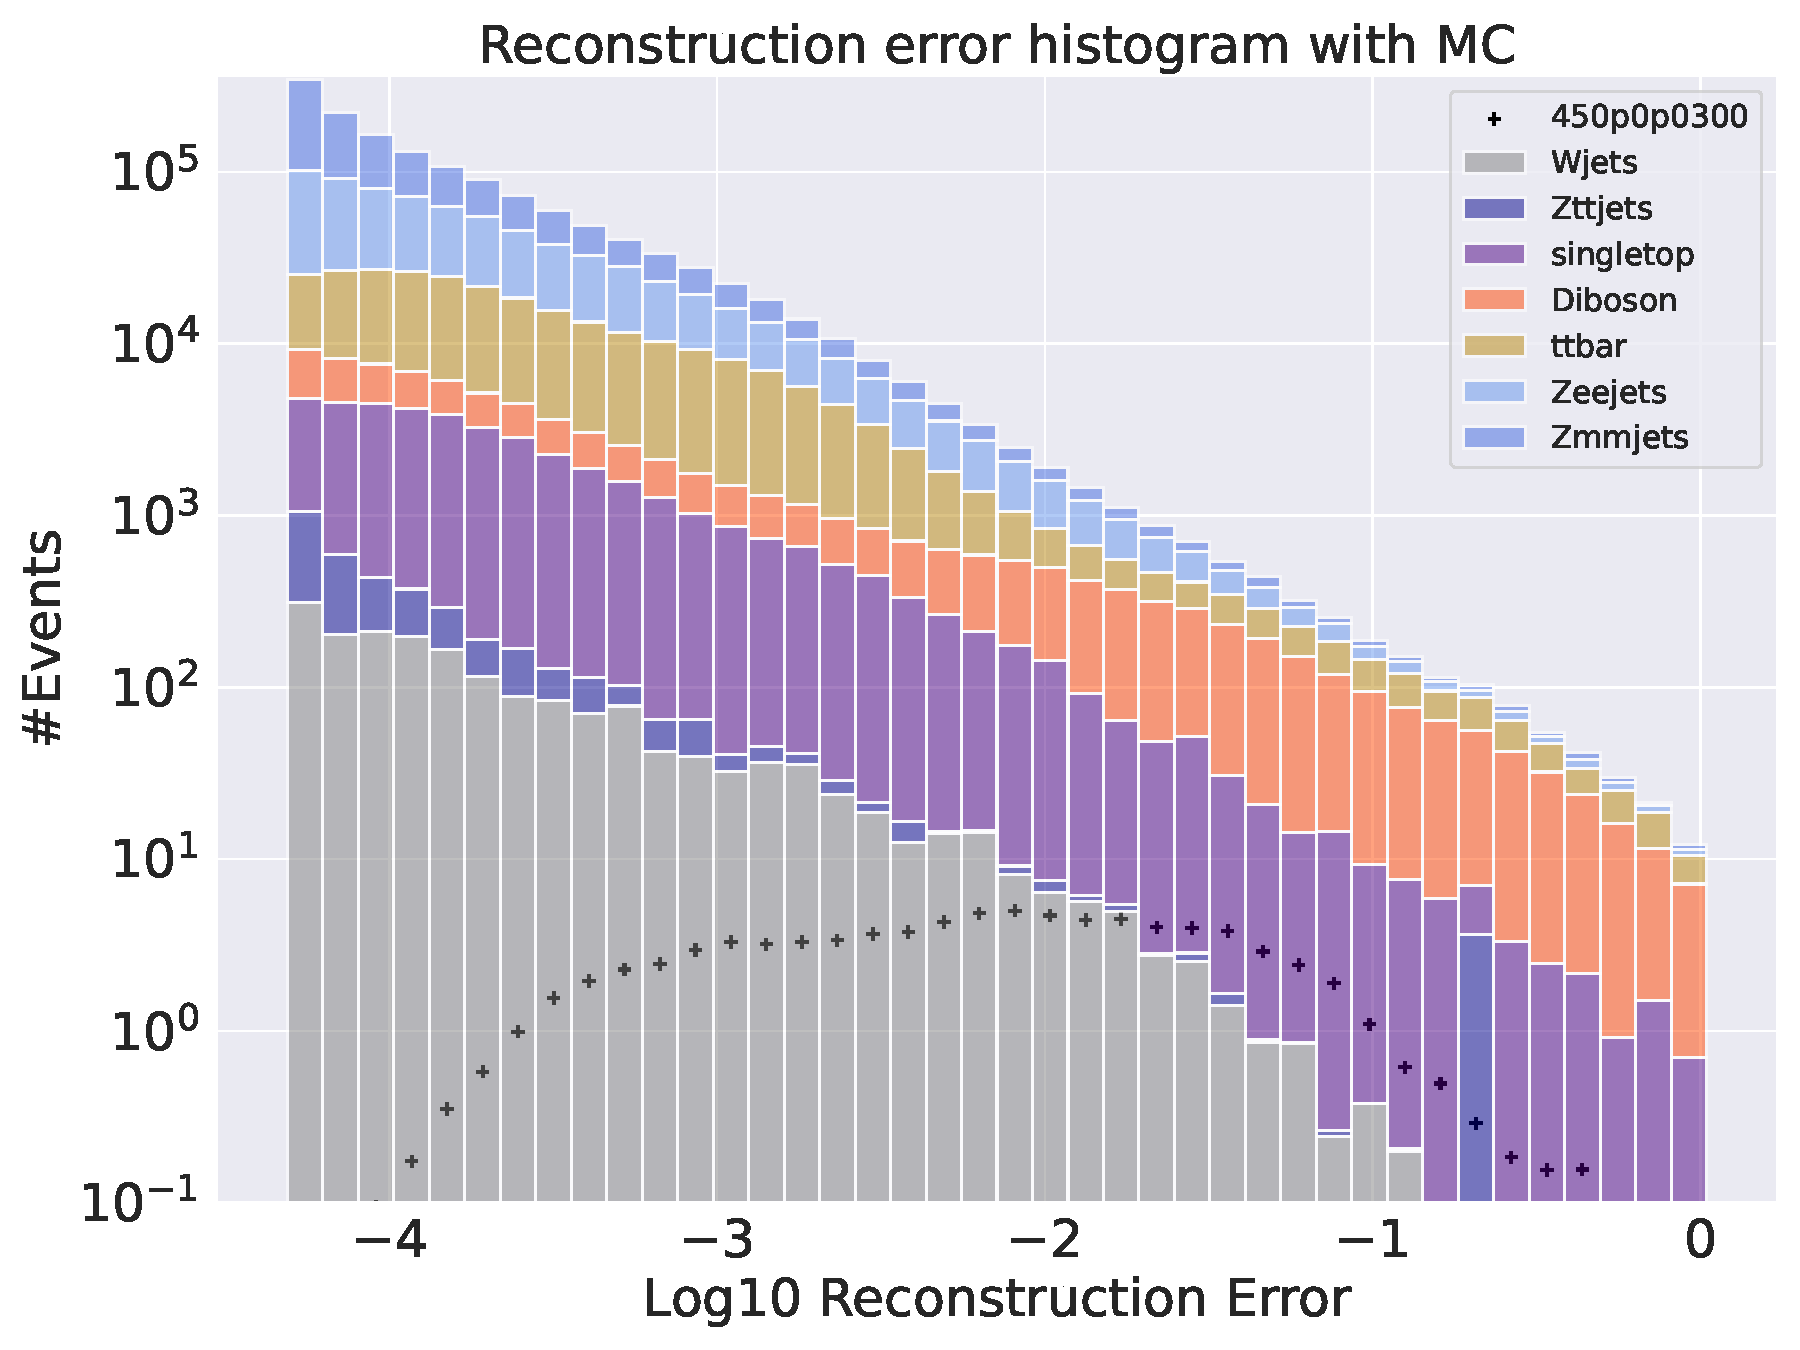
\includegraphics[width=\textwidth]{Figures/AE_testing/small/2lep/b_data_recon_big_rm3_feats_sig_450p0p0300_.pdf}
        \caption{ }
        \label{fig:AE_2lep_big_450}
    \end{subfigure}
    \hfill
    \begin{subfigure}{.49\textwidth}
        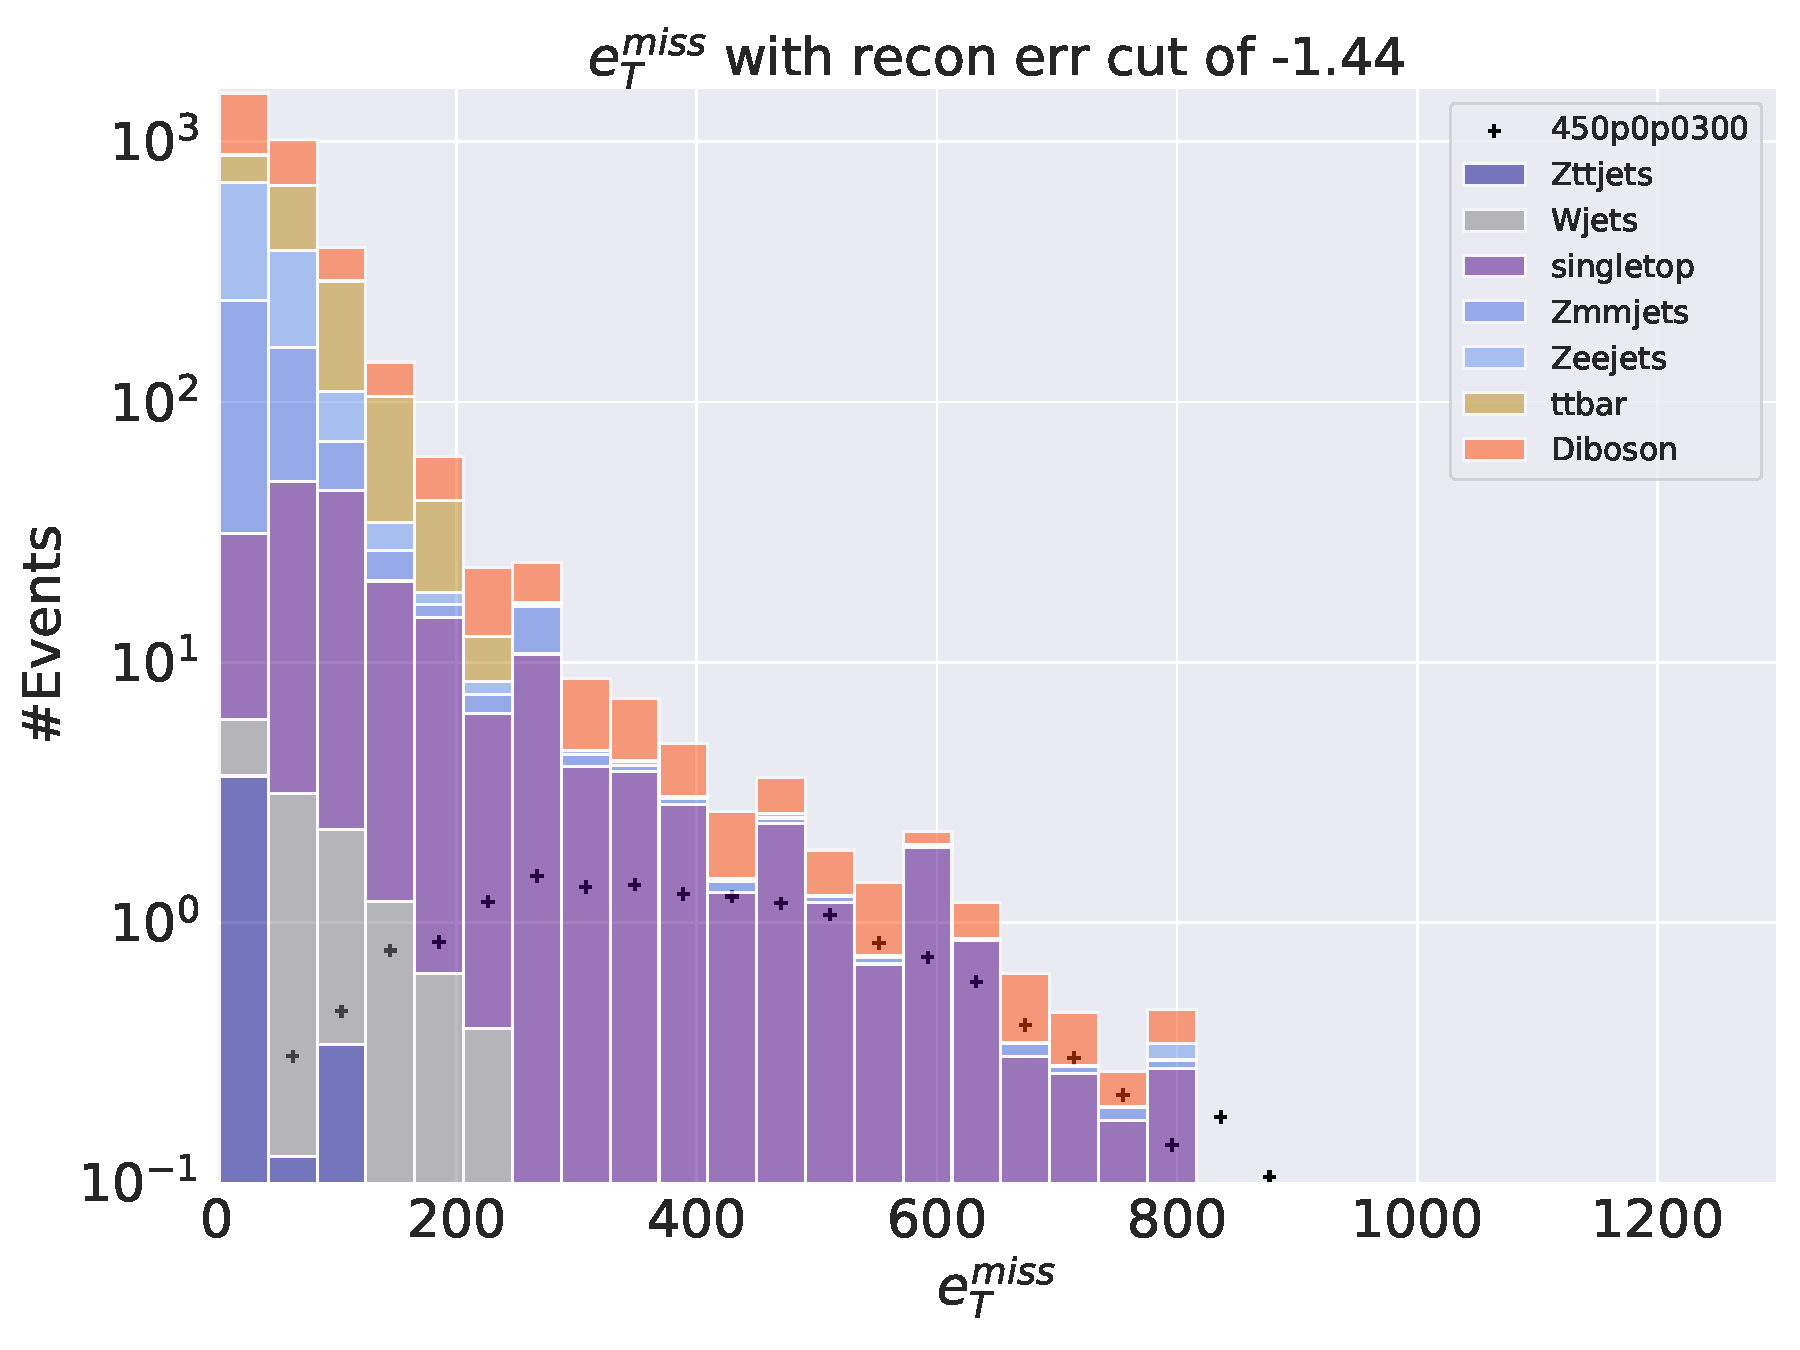
\includegraphics[width=\textwidth]{Figures/AE_testing/big/2lep/b_data_recon_big_rm3_feats_sig_450p0p0300_recon_errcut_-1.44.pdf}
        \caption{}
        \label{fig:AE_2lep_big_etmiss_450}
    \end{subfigure}
    \hfill 
    \begin{subfigure}{.49\textwidth}
        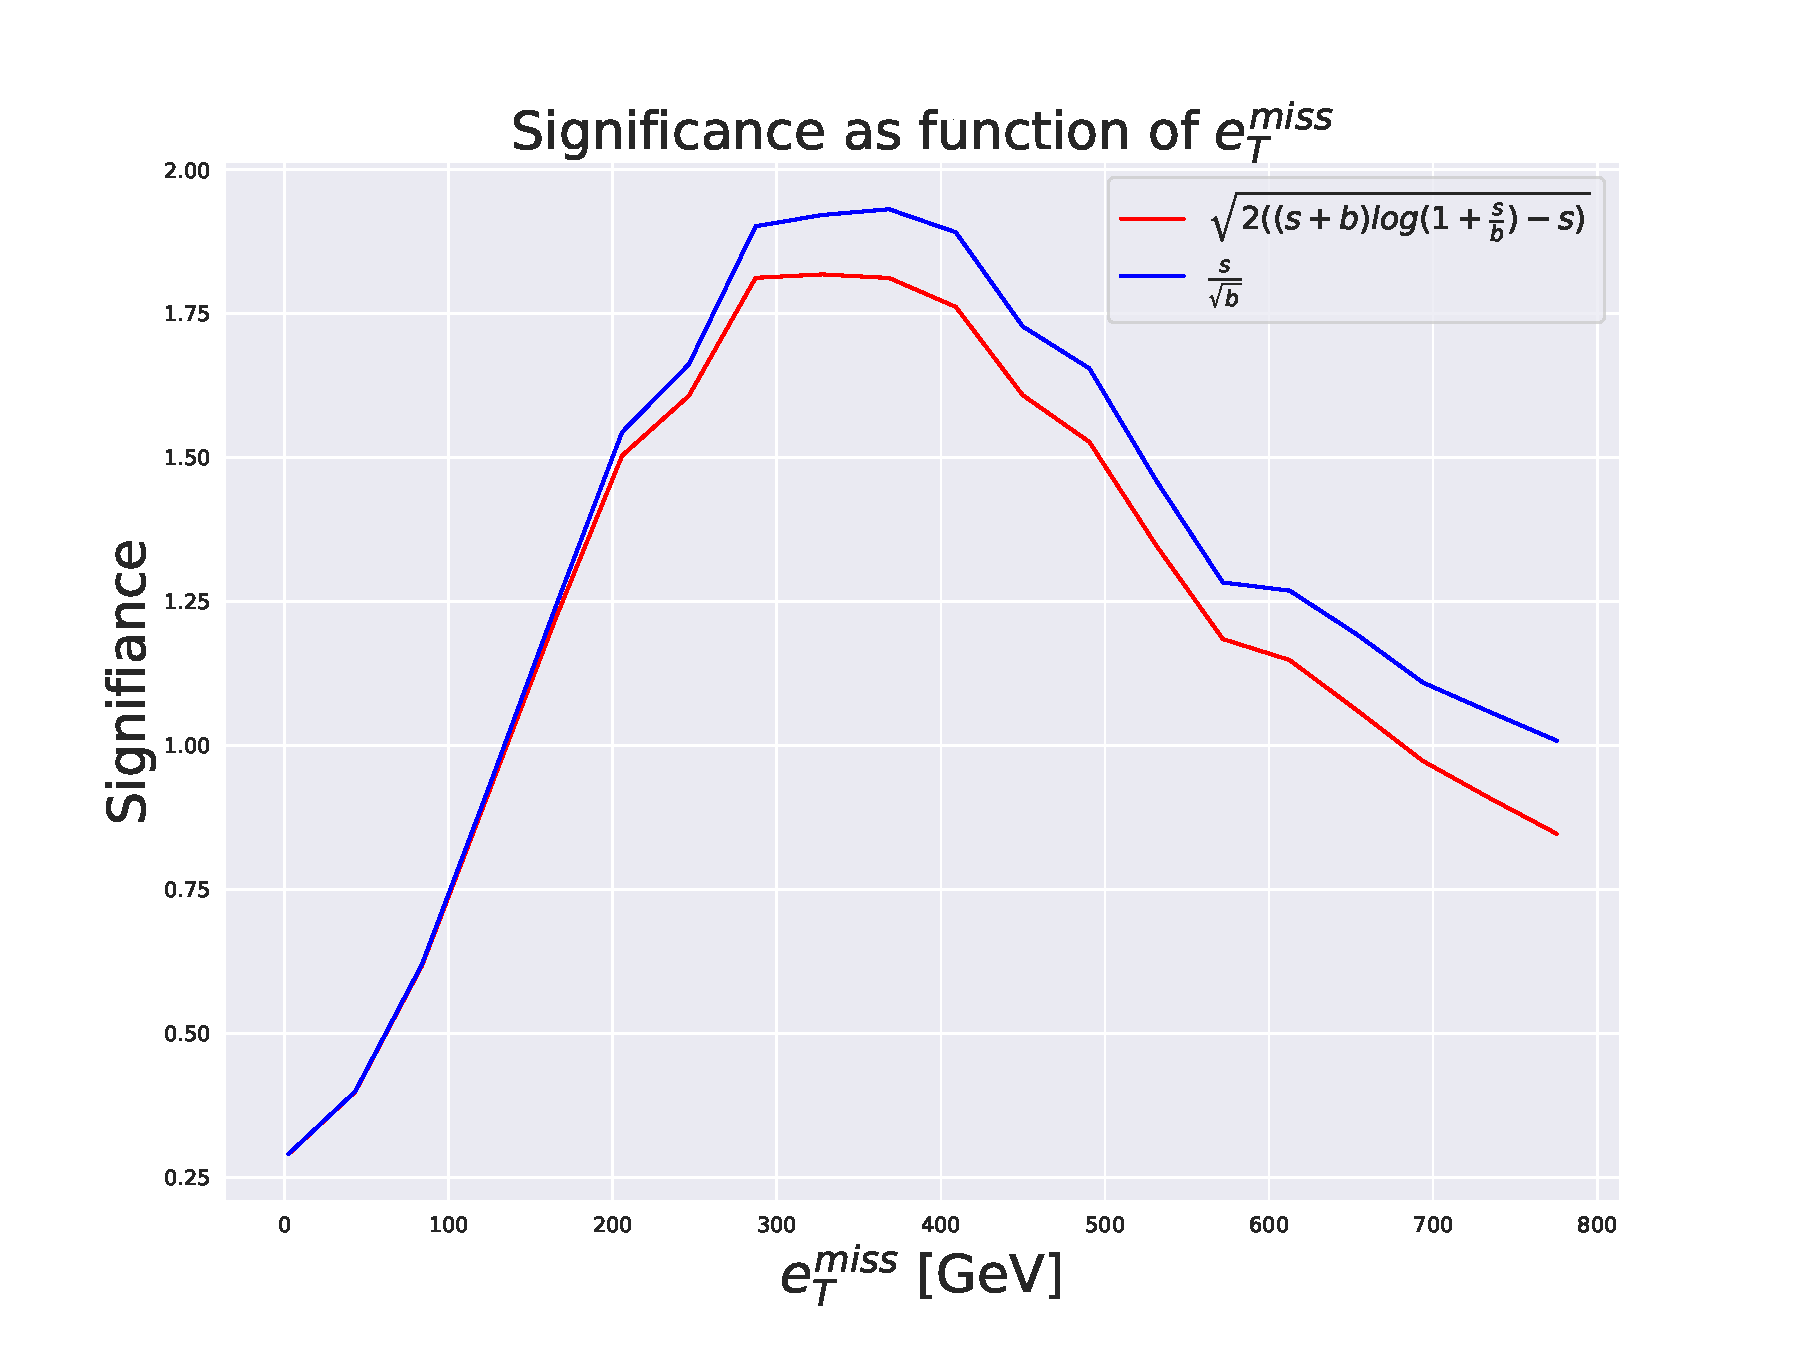
\includegraphics[width=\textwidth]{Figures/AE_testing/big/2lep/significance_etmiss_450p0p0300_-1.4360553938127363.pdf}
        \caption{}
        \label{fig:AE_2lep_big_signi_450}
    \end{subfigure}
    \hfill      
    \caption[2lep deep network | $450p300$ | AE]{Reconstruction error (a), $e_T^{miss}$ signal region (b) and significance as function of 
    $e_T^{miss}$ (c) for the deep regular autoencoder using SUSY $450p300$. 
    (a) shows the reconstruction error distribution for the SM MC and the SUSY signal. 
    The autoencoder produces a slope-like shape that is highly shifted to the lower end of the reconstruction error range
for the background. The signal is more evenly spread out along the x-axis. The peaks of the two distributions are totally separated
with two orders of magnitude in reconstruction error. (b) shows the $e_T^{miss}$
T distribution for the SM MC and the SUSY signal in the signal region. The signal region is made using a cut around
$10^{-1.44}$. Most of the background is removed, and the peaks of the SM MC and signal distributions are
somewhat separated. (c) shows the significance as function of $e_T^{miss}$. The peak is put 
around a cut of about 380 GeV in the $e_T^{miss}$, with a significance of around $1.85$.}
    \label{fig:AE_2lep_big_rec_sig_signi_450}
\end{figure}



\begin{figure}[h!]
    \centering
    \begin{subfigure}{.49\textwidth}
        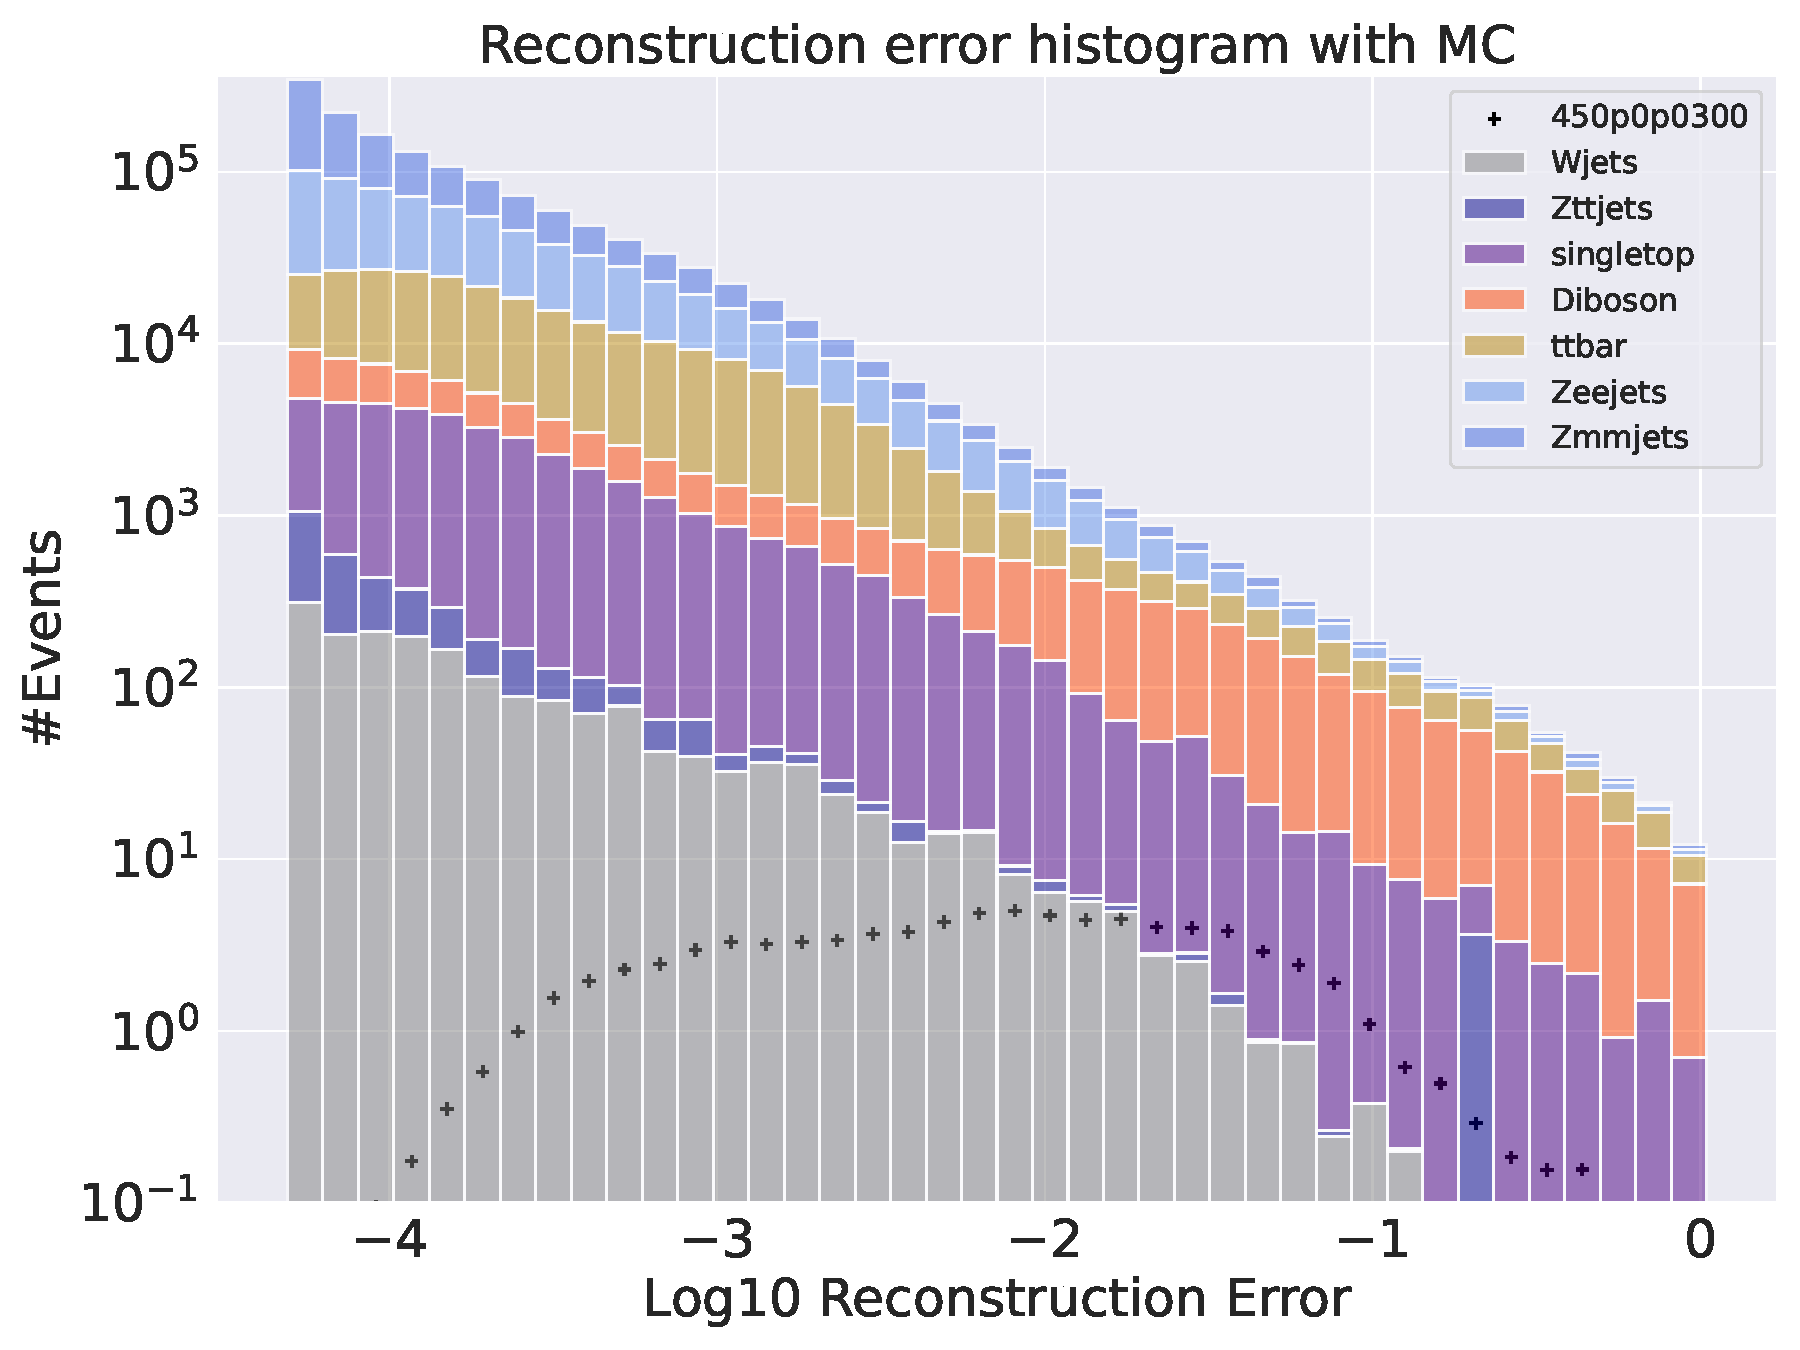
\includegraphics[width=\textwidth]{Figures/AE_testing/small/2lep/b_data_recon_big_rm3_feats_sig_450p0p0300_.pdf}
        \caption{ }
        \label{fig:AE_2lep_small_450}
    \end{subfigure}
    \hfill
    \begin{subfigure}{.49\textwidth}
        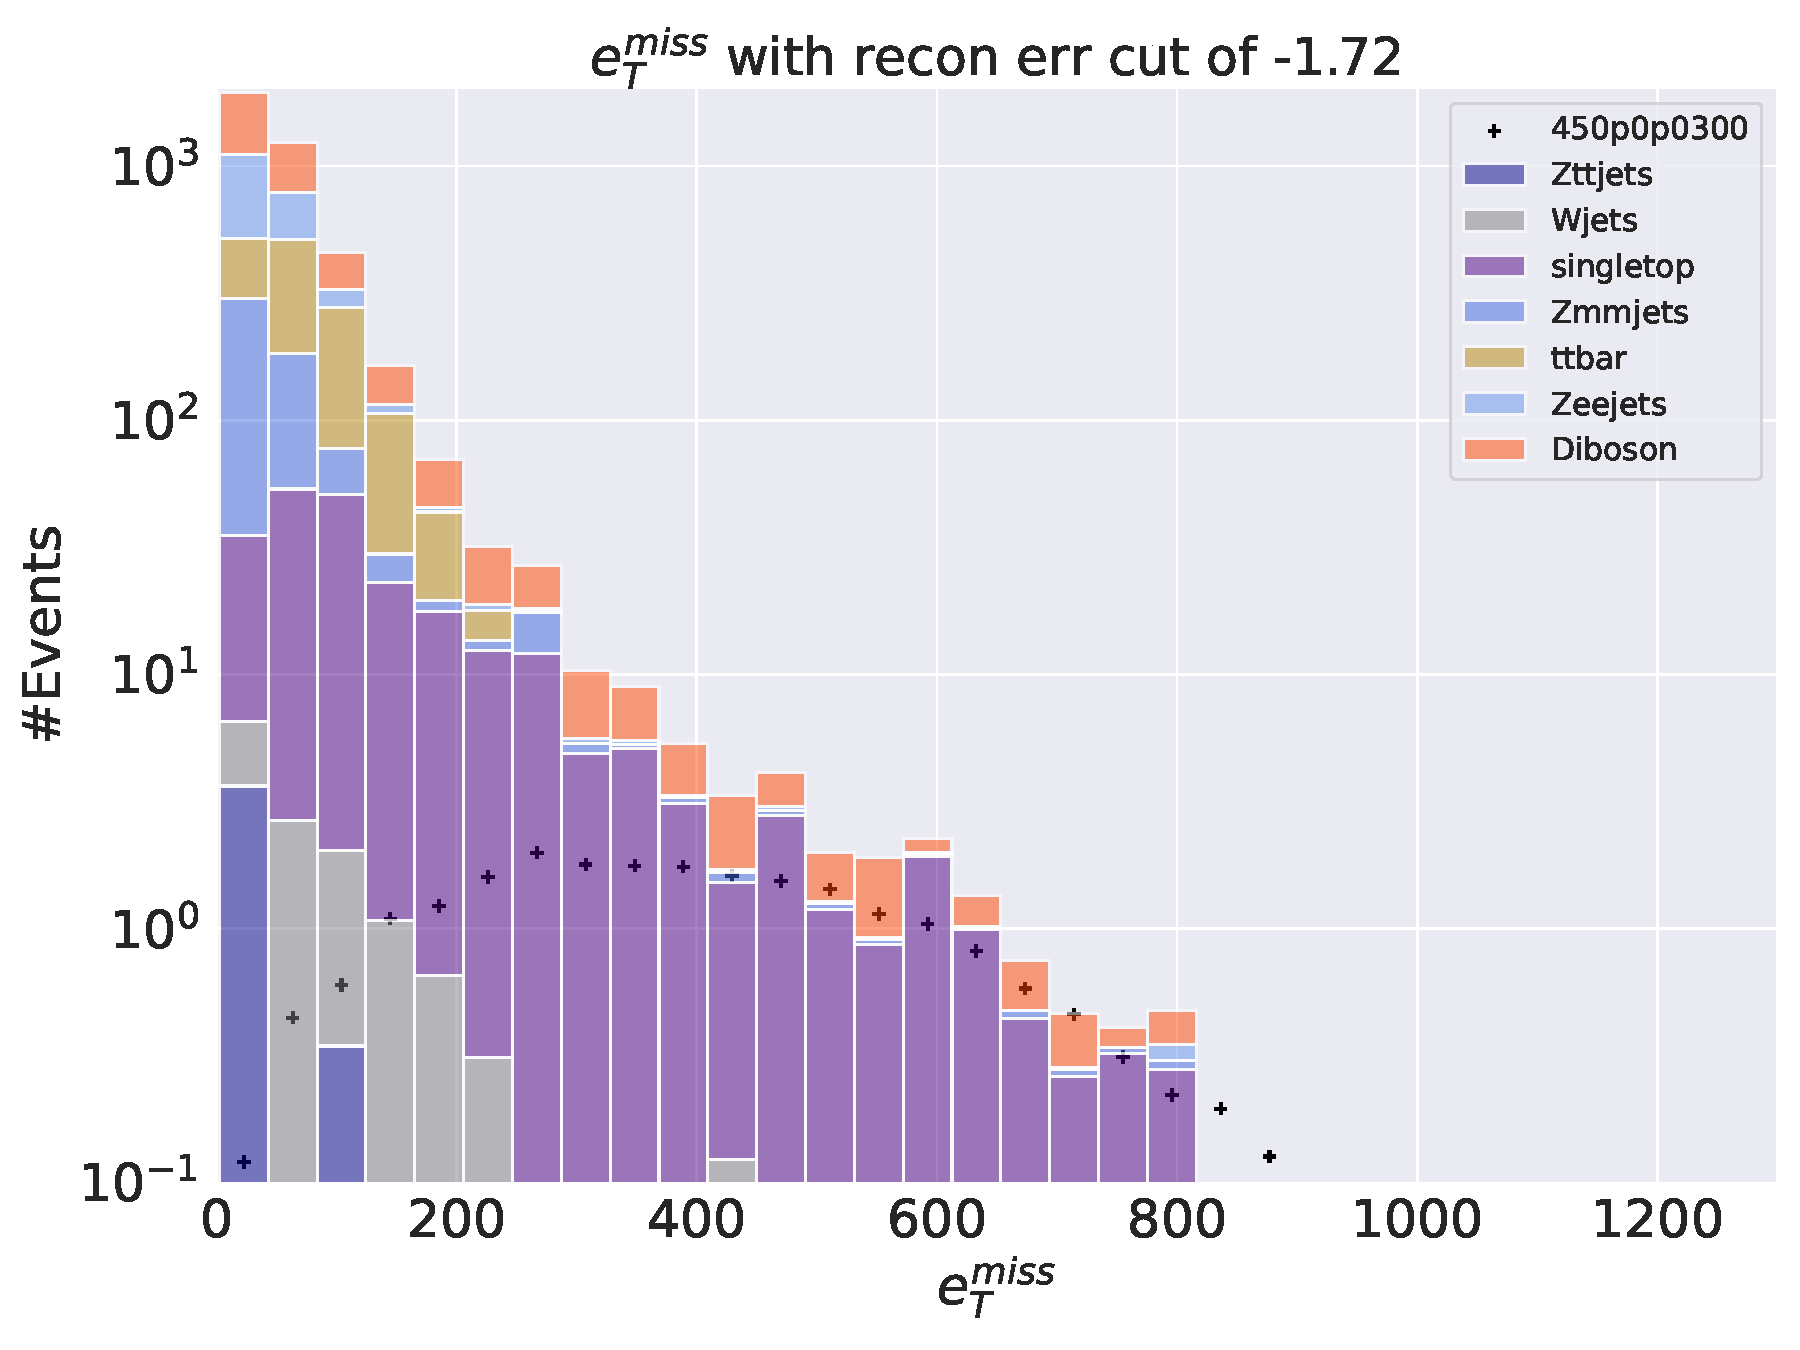
\includegraphics[width=\textwidth]{Figures/AE_testing/small/2lep/b_data_recon_big_rm3_feats_sig_450p0p0300_recon_errcut_-1.72.pdf}
        \caption{}
        \label{fig:AE_2lep_small_etmiss_450}
    \end{subfigure}
    \hfill  
    \begin{subfigure}{.49\textwidth}
        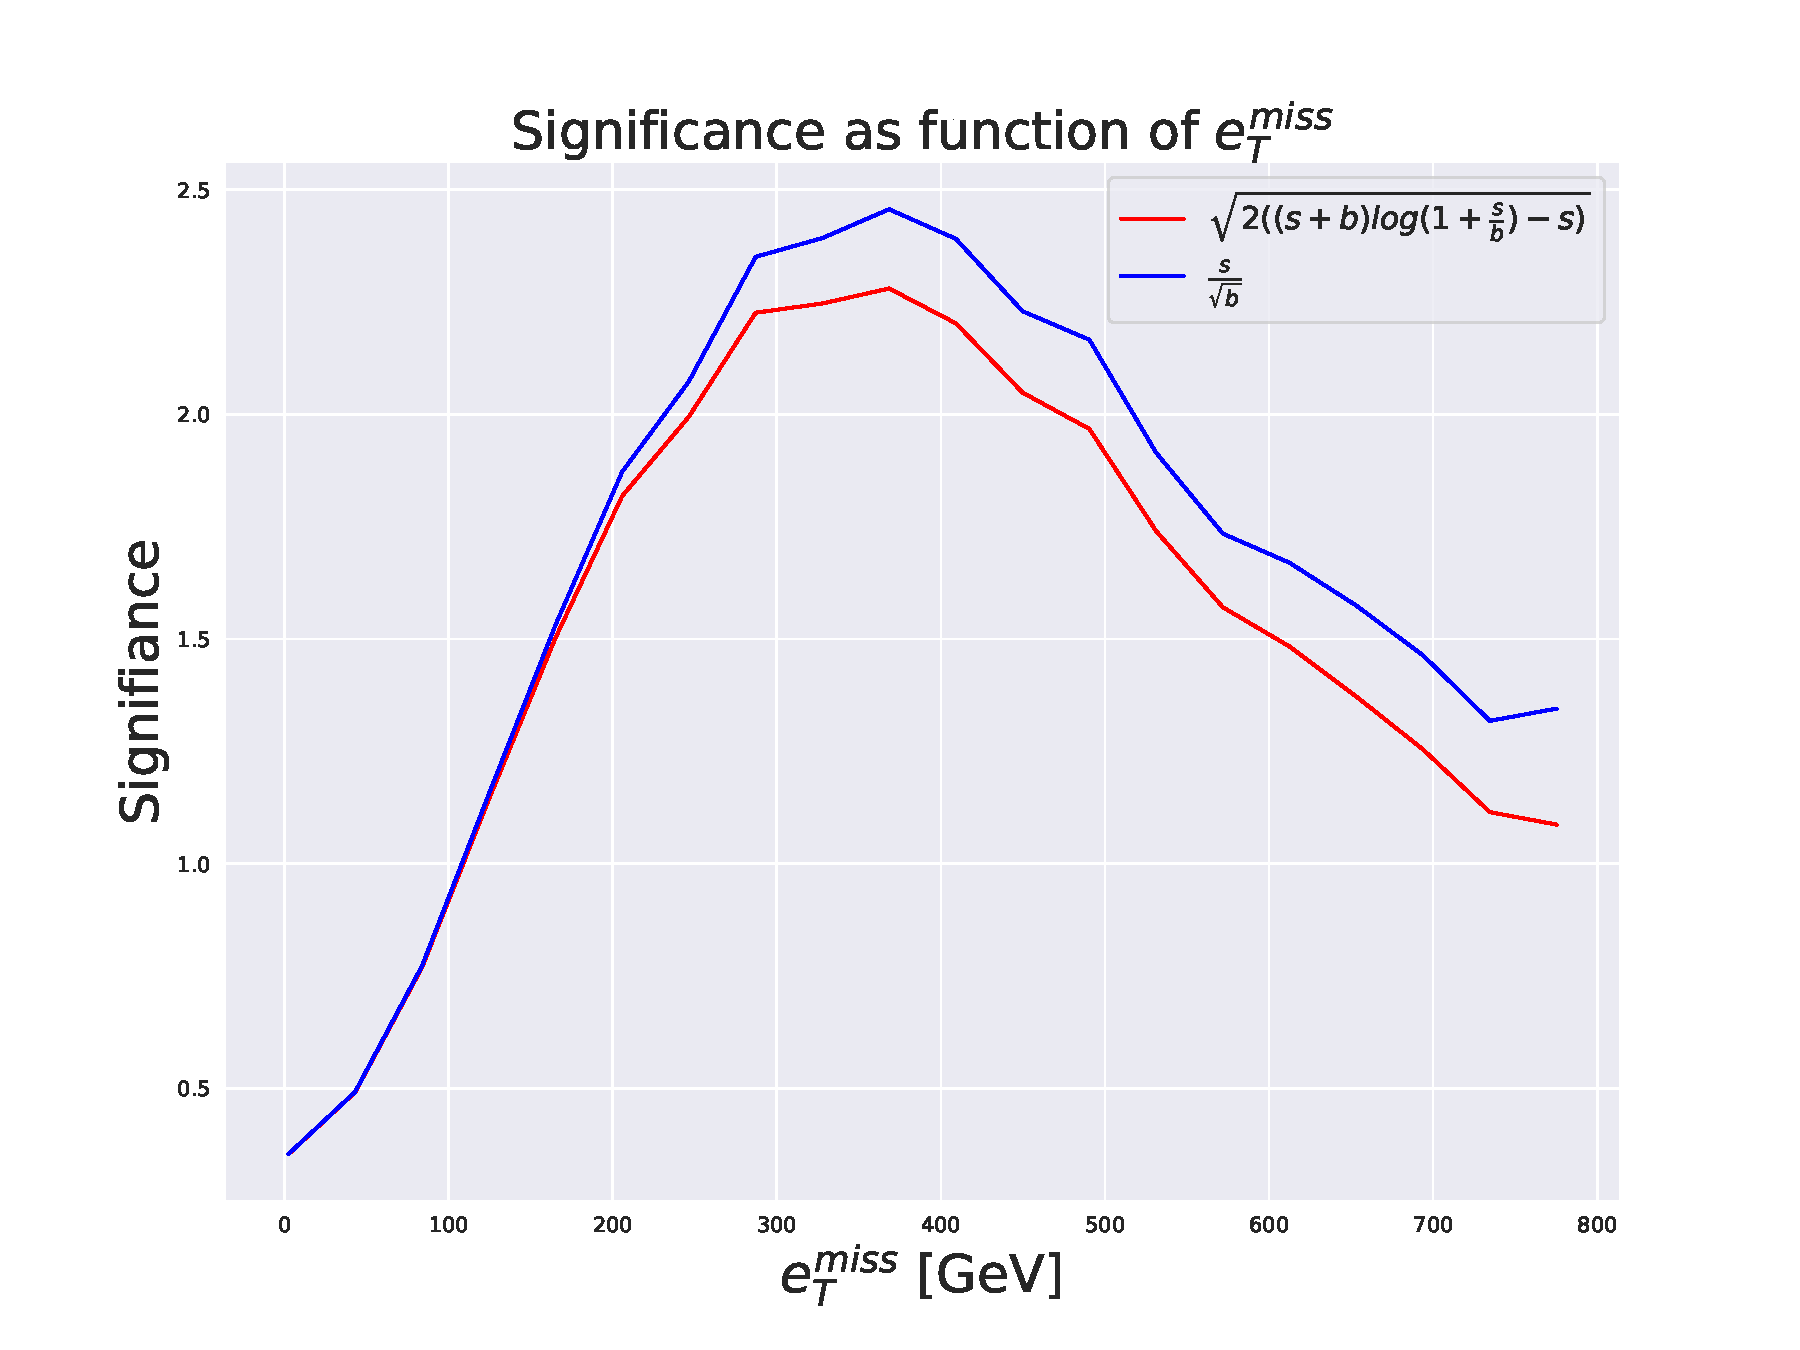
\includegraphics[width=\textwidth]{Figures/AE_testing/small/2lep/significance_etmiss_450p0p0300_-1.7167506533614734.pdf}
        \caption{}
        \label{fig:AE_2lep_small_signi_450}
    \end{subfigure}
    \hfill      
    \caption[2lep shallow network | $450p300$ | AE]{Reconstruction error (a), $e_T^{miss}$ signal region (b) and significance as function of 
    $e_T^{miss}$ (c) for the shallow regular autoencoder using SUSY $450p300$. 
    (a) shows the reconstruction error distribution for the SM MC and the SUSY signal. 
    The autoencoder produces a slope-like shape that is highly shifted to the lower end of the reconstruction error range
for the background. The signal is more evenly spread out along the x-axis. The peaks of the two distributions are totally separated
with two orders of magnitude in reconstruction error. (b) shows the $e_T^{miss}$
T distribution for the SM MC and the SUSY signal in the signal region. The signal region is made using a cut around
$10^{-1.72}$. Most of the background is removed, and the peaks of the SM MC and signal distributions are
somewhat separated. (c) shows the significance as function of $e_T^{miss}$. The peak is put 
around a cut of about 380 GeV in the $e_T^{miss}$, with a significance of around $2.4$.}
    \label{fig:AE_2lep_small_rec_sig_signi_450}
\end{figure}


\begin{figure}[h!]
    \centering
    \begin{subfigure}{.49\textwidth}
        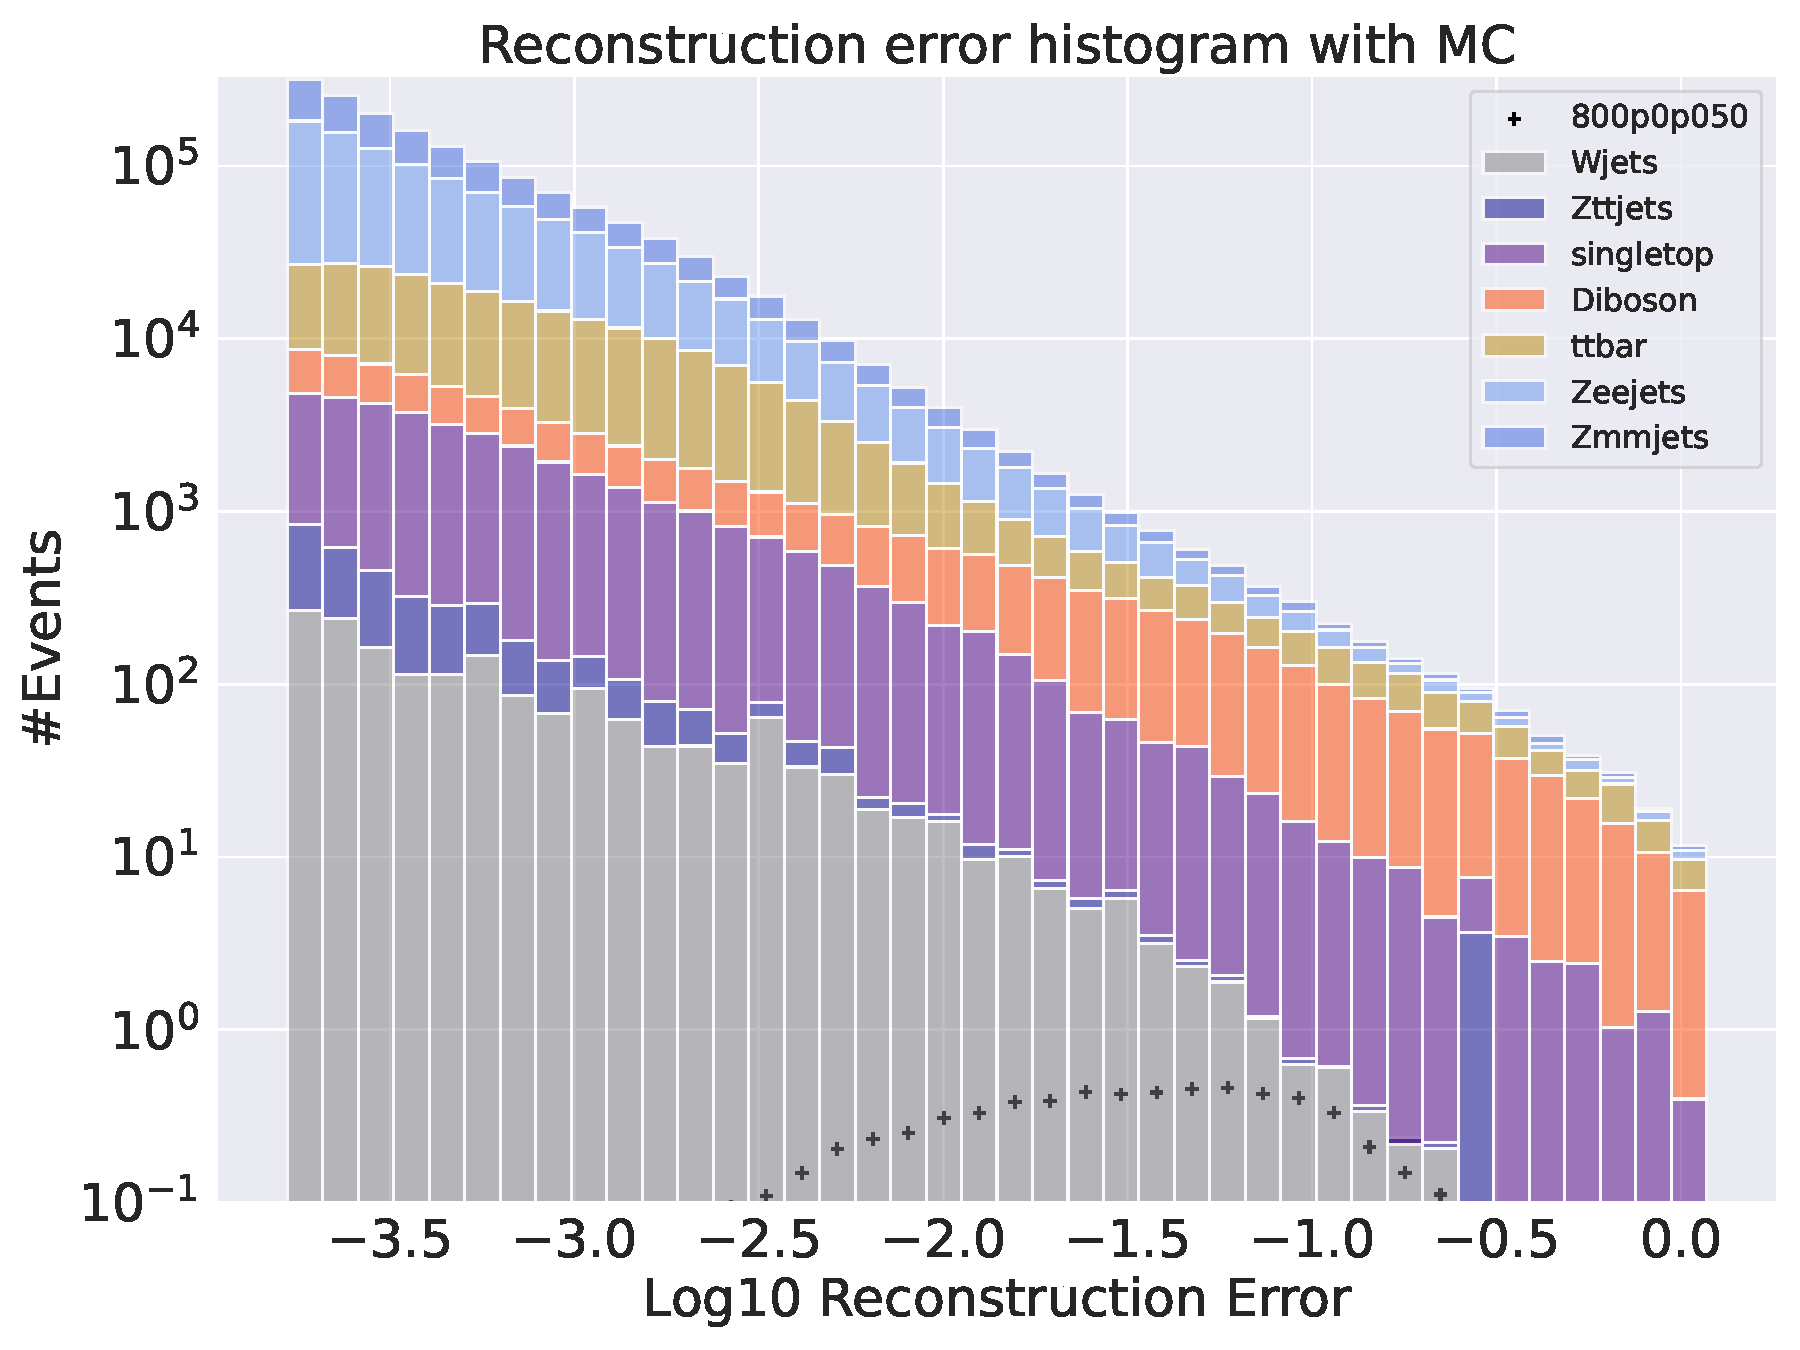
\includegraphics[width=\textwidth]{Figures/AE_testing/big/2lep/b_data_recon_big_rm3_feats_sig_800p0p050_.pdf}
        \caption{ }
        \label{fig:AE_2lep_big_800}
    \end{subfigure}
    \hfill
    \begin{subfigure}{.49\textwidth}
        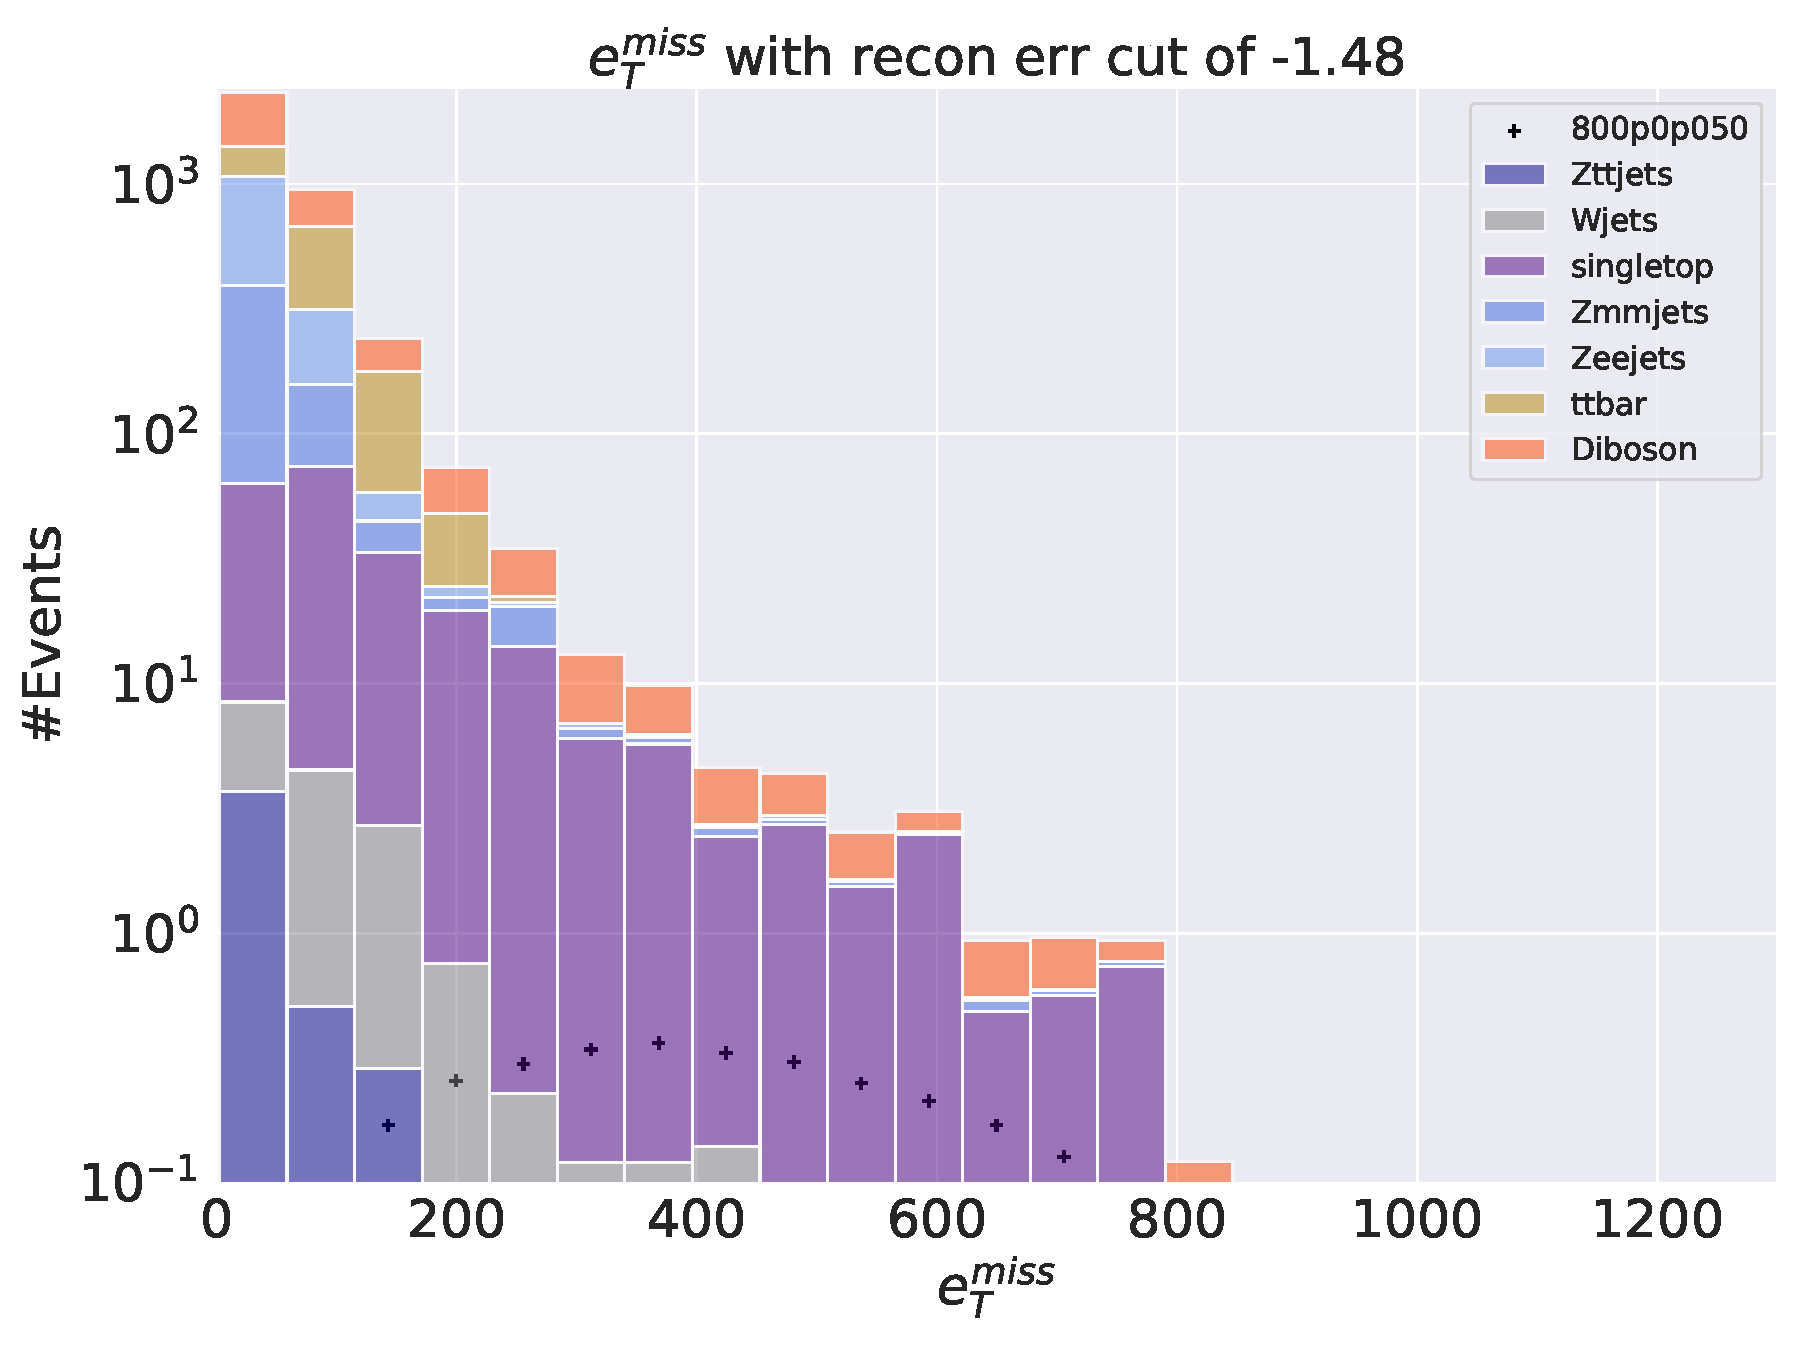
\includegraphics[width=\textwidth]{Figures/AE_testing/big/2lep/b_data_recon_big_rm3_feats_sig_800p0p050_recon_errcut_-1.48.pdf}
        \caption{}
        \label{fig:AE_2lep_big_etmiss_800}
    \end{subfigure}
    \hfill
      
    \begin{subfigure}{.49\textwidth}
        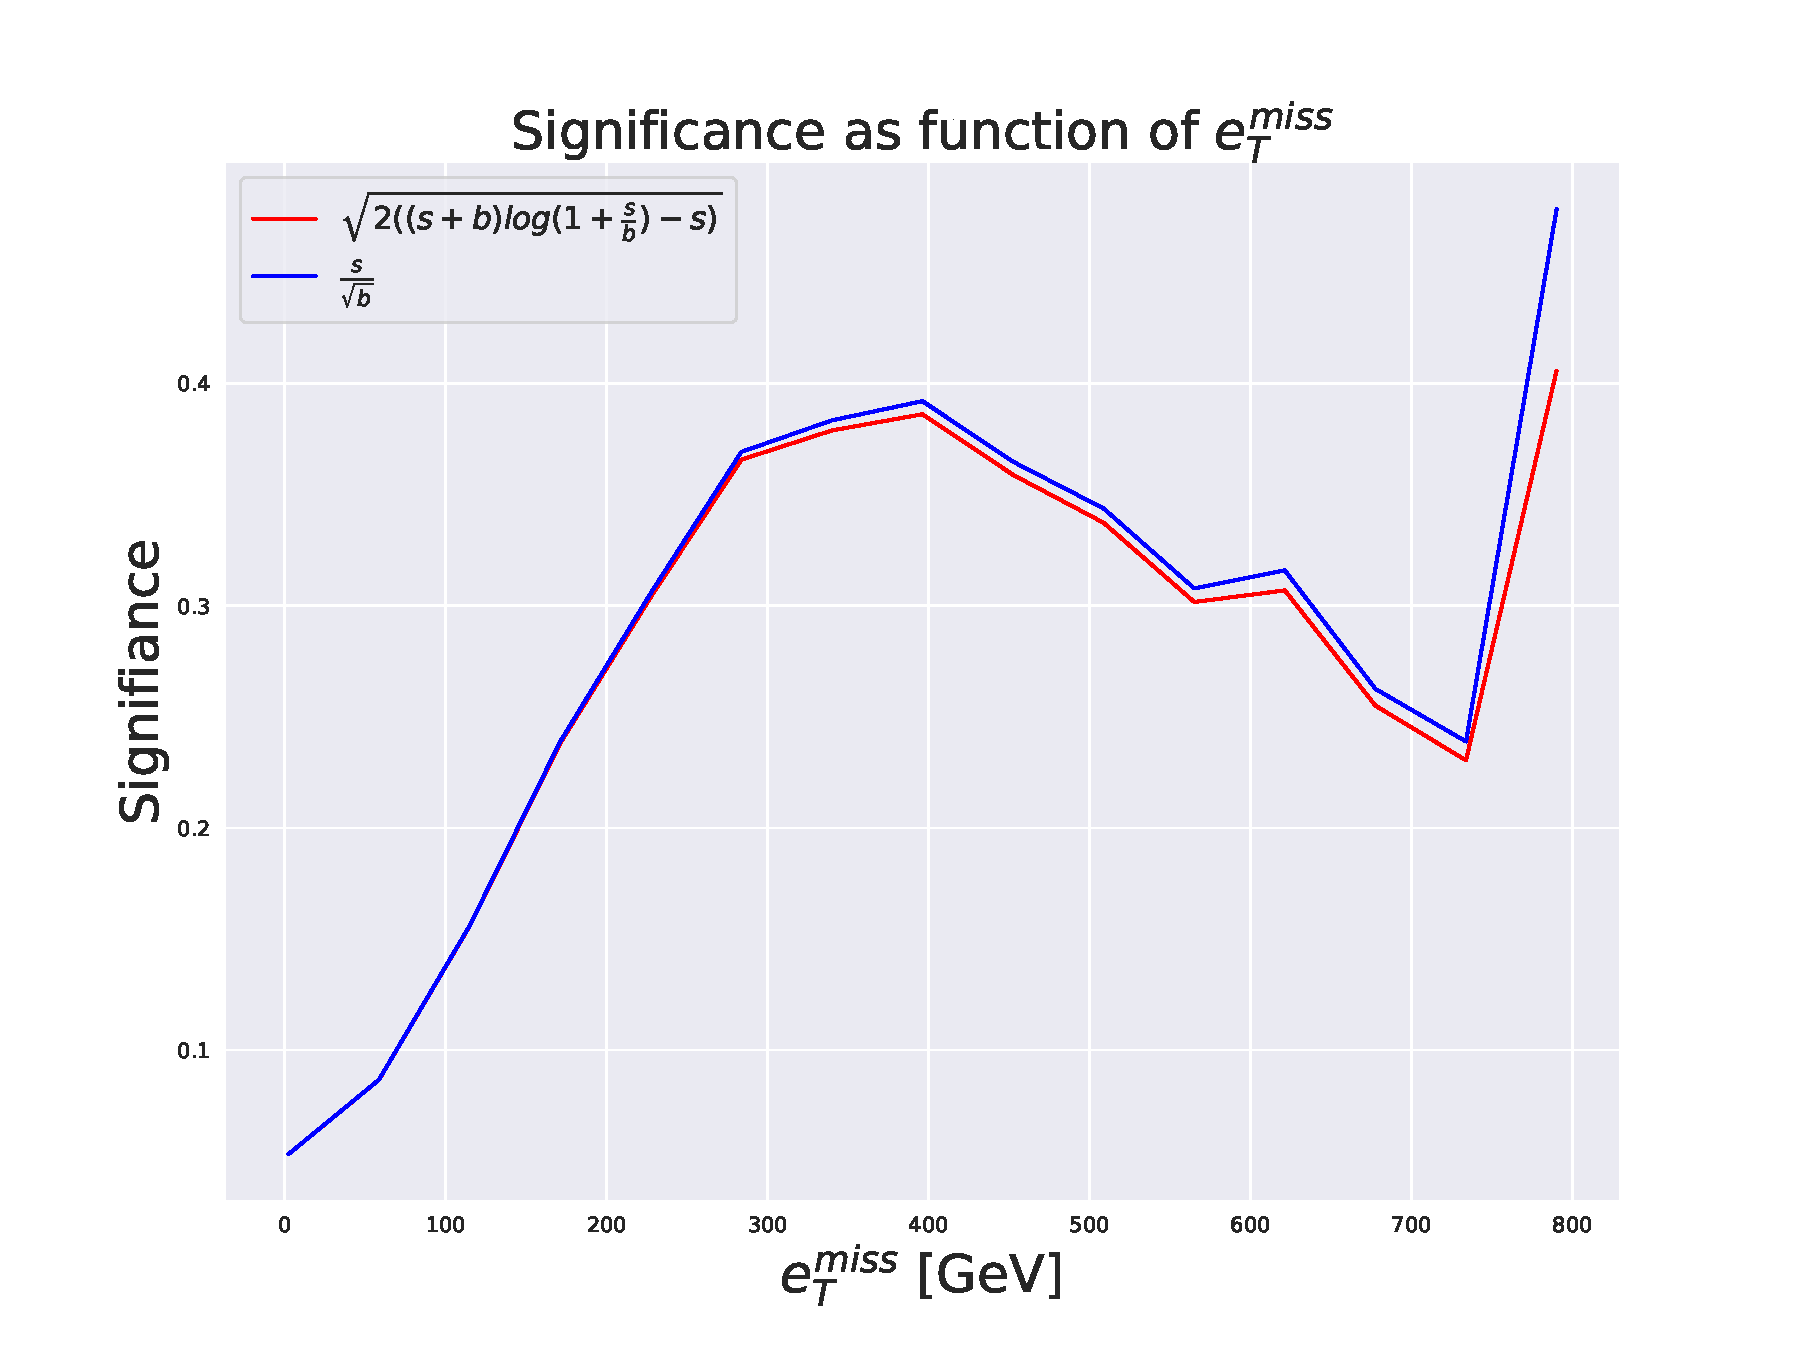
\includegraphics[width=\textwidth]{Figures/AE_testing/big/2lep/significance_etmiss_800p0p050_-1.4833711230716062.pdf}
        \caption{}
        \label{fig:AE_2lep_big_signi_800}
    \end{subfigure}
    \hfill      
    \caption[2lep deep network | $800p50$ | AE]{Reconstruction error (a), $e_T^{miss}$ signal region (b) and significance as function of 
    $e_T^{miss}$ (c) for the deep regular autoencoder using SUSY $800p50$. 
    Figure \ref{fig:AE_2lep_big_800} shows the reconstruction error distribution for the SM MC and the SUSY signal. 
Here the autoencoder produce slope-like shape that is highly shifted to the lower end of the reconstruction error range
for the background. The signal has a peak around $10^{-1.5}$ with a mirrored distribution shape from the background. The peaks of the two distributions are separated
with two orders of magnitude in reconstruction error. Figure \ref{fig:AE_2lep_big_etmiss_800} shows the $e_T^{miss}$
T distribution for the SM MC and the SUSY signal in the signal region. The signal region is made using a cut around
$10^{-1.48}$. Most of the background is removed, and the peaks of the SM MC and signal distributions are
somewhat separated.  Figure \ref{fig:AE_2lep_big_signi_800} shows the significance as function of $e_T^{miss}$. The peak is put 
around a cut of about 400 GeV in the $e_T^{miss}$, with a significance of around $0.38$.}
    \label{fig:AE_2lep_big_rec_sig_signi_800}
\end{figure}

\begin{figure}[h!]
    \centering
    \begin{subfigure}{.49\textwidth}
        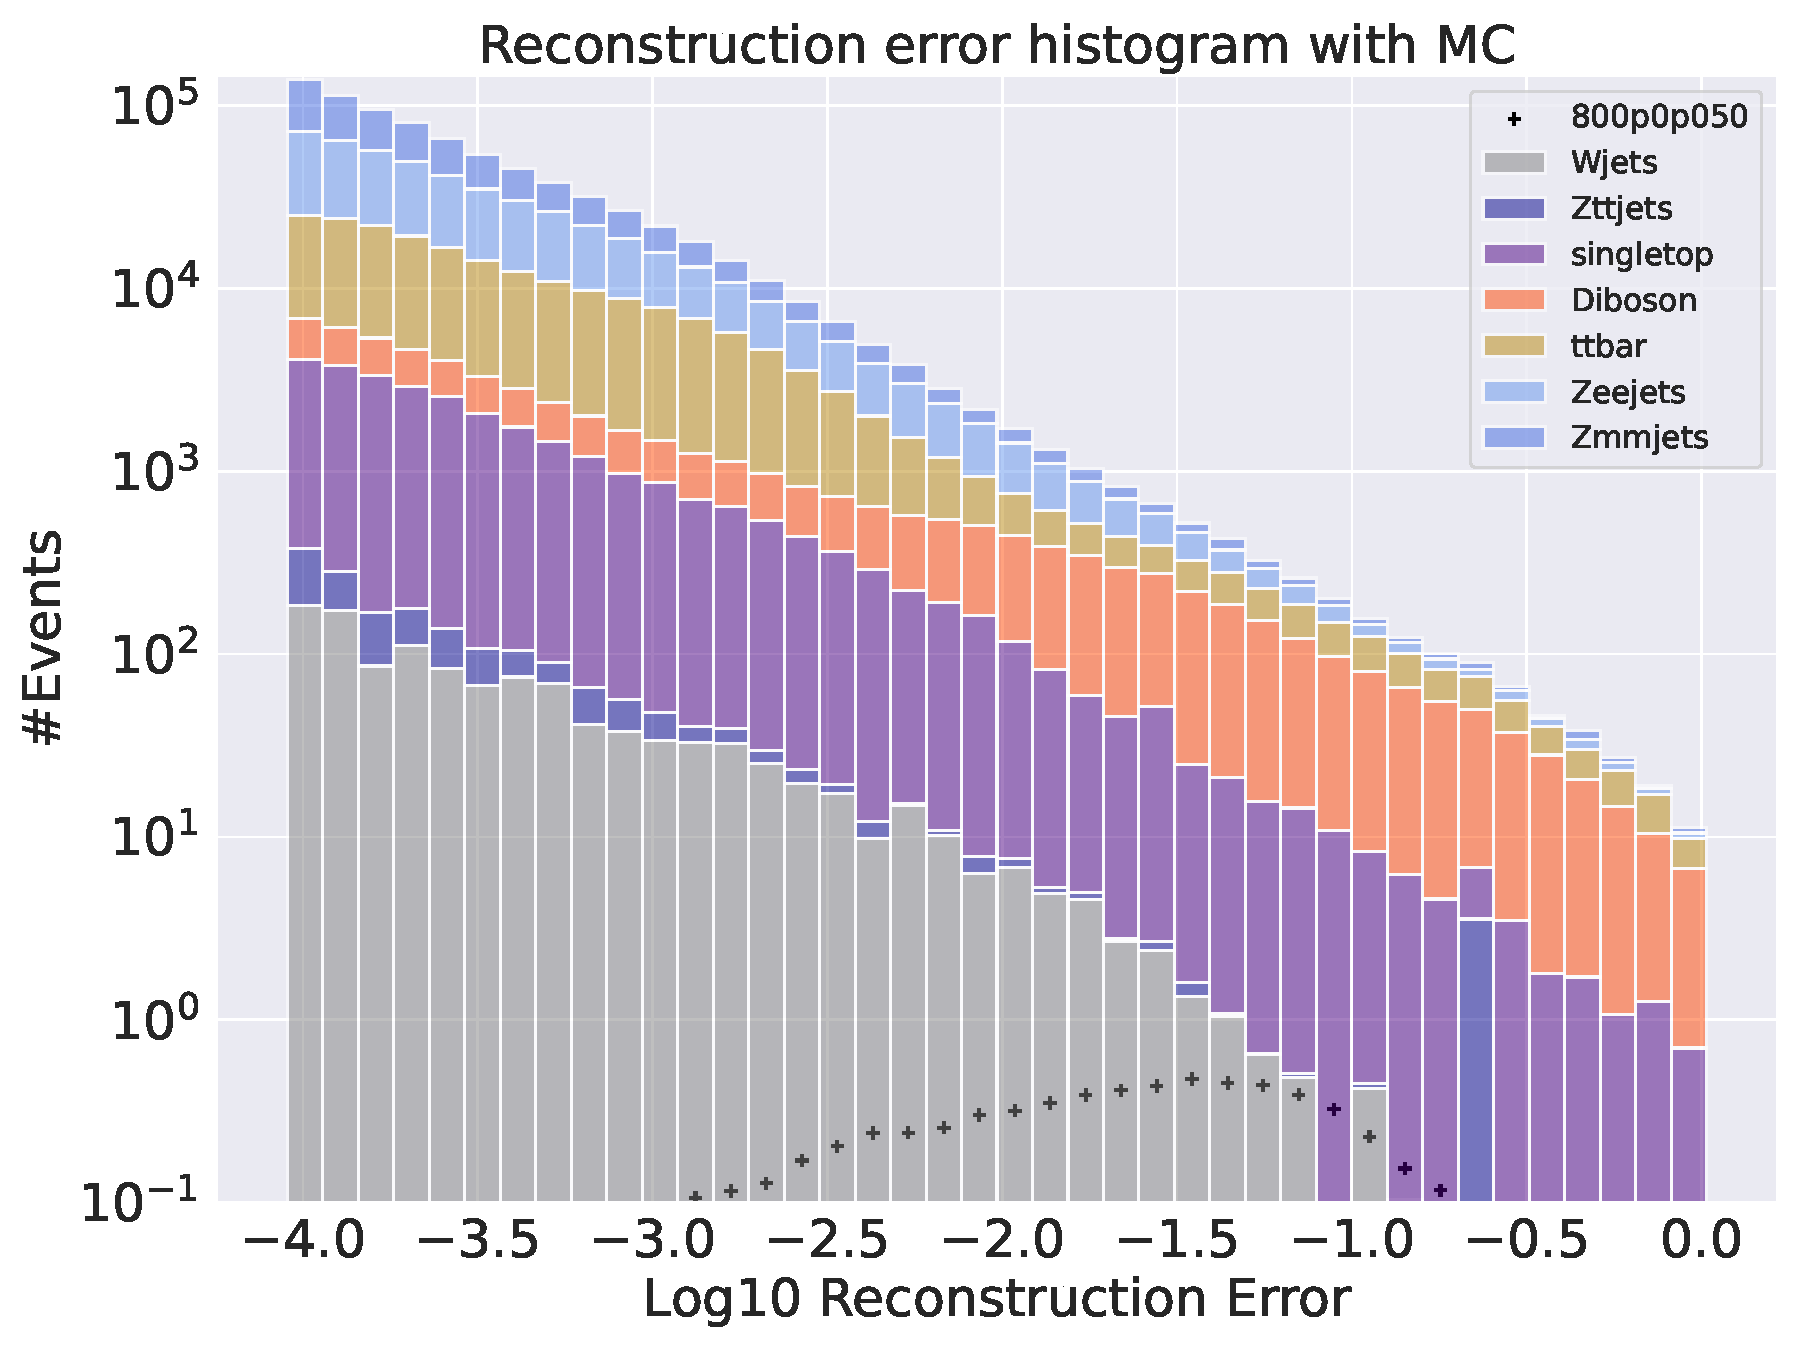
\includegraphics[width=\textwidth]{Figures/AE_testing/small/2lep/b_data_recon_big_rm3_feats_sig_800p0p050_.pdf}
        \caption{ }
        \label{fig:AE_2lep_small_800}
    \end{subfigure}
    \hfill
    \begin{subfigure}{.49\textwidth}
        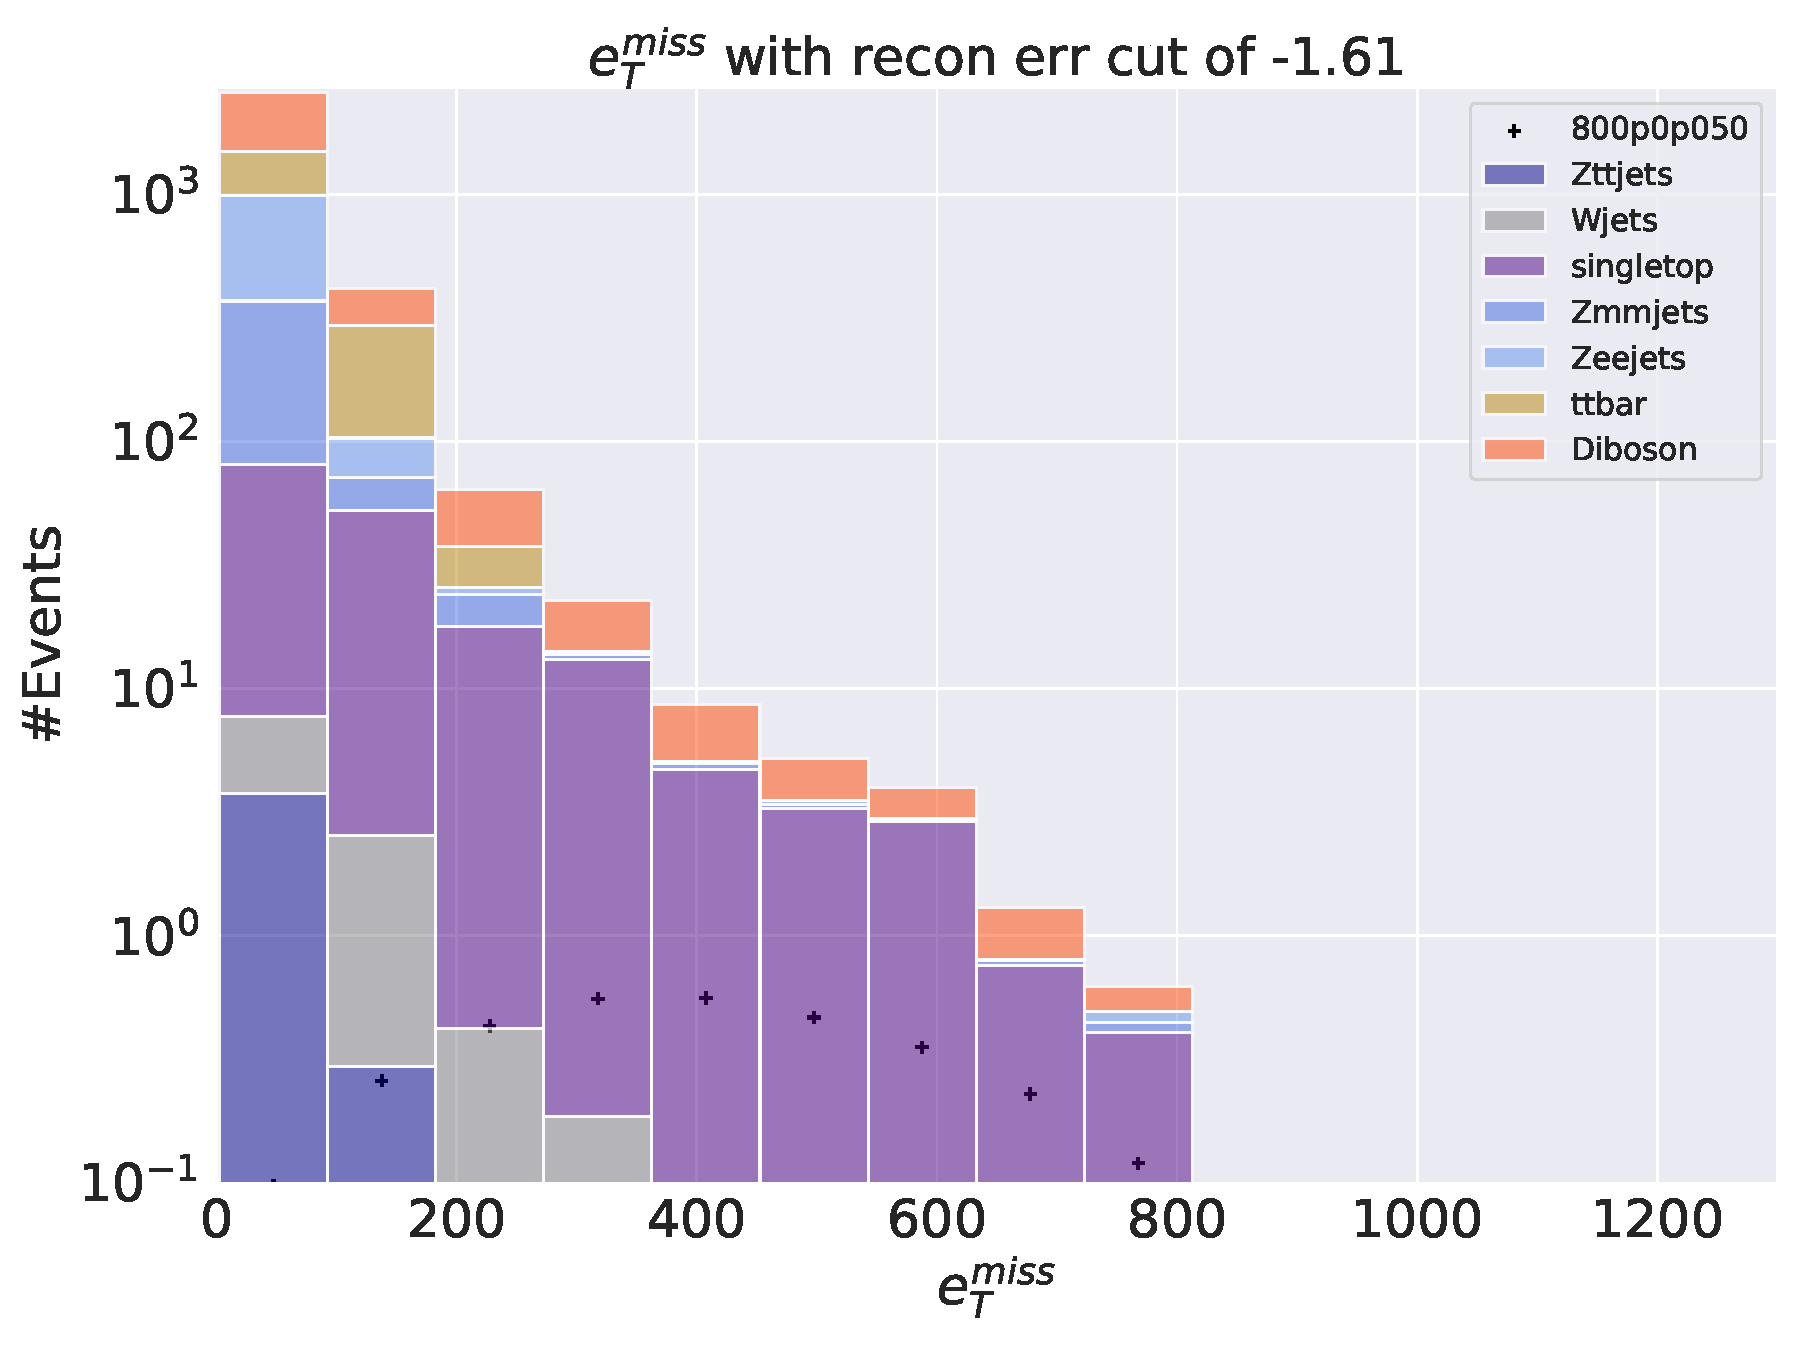
\includegraphics[width=\textwidth]{Figures/AE_testing/small/2lep/b_data_recon_big_rm3_feats_sig_800p0p050_recon_errcut_-1.61.pdf}
        \caption{}
        \label{fig:AE_2lep_small_etmiss_800}
    \end{subfigure}
    \hfill  
    \begin{subfigure}{.49\textwidth}
        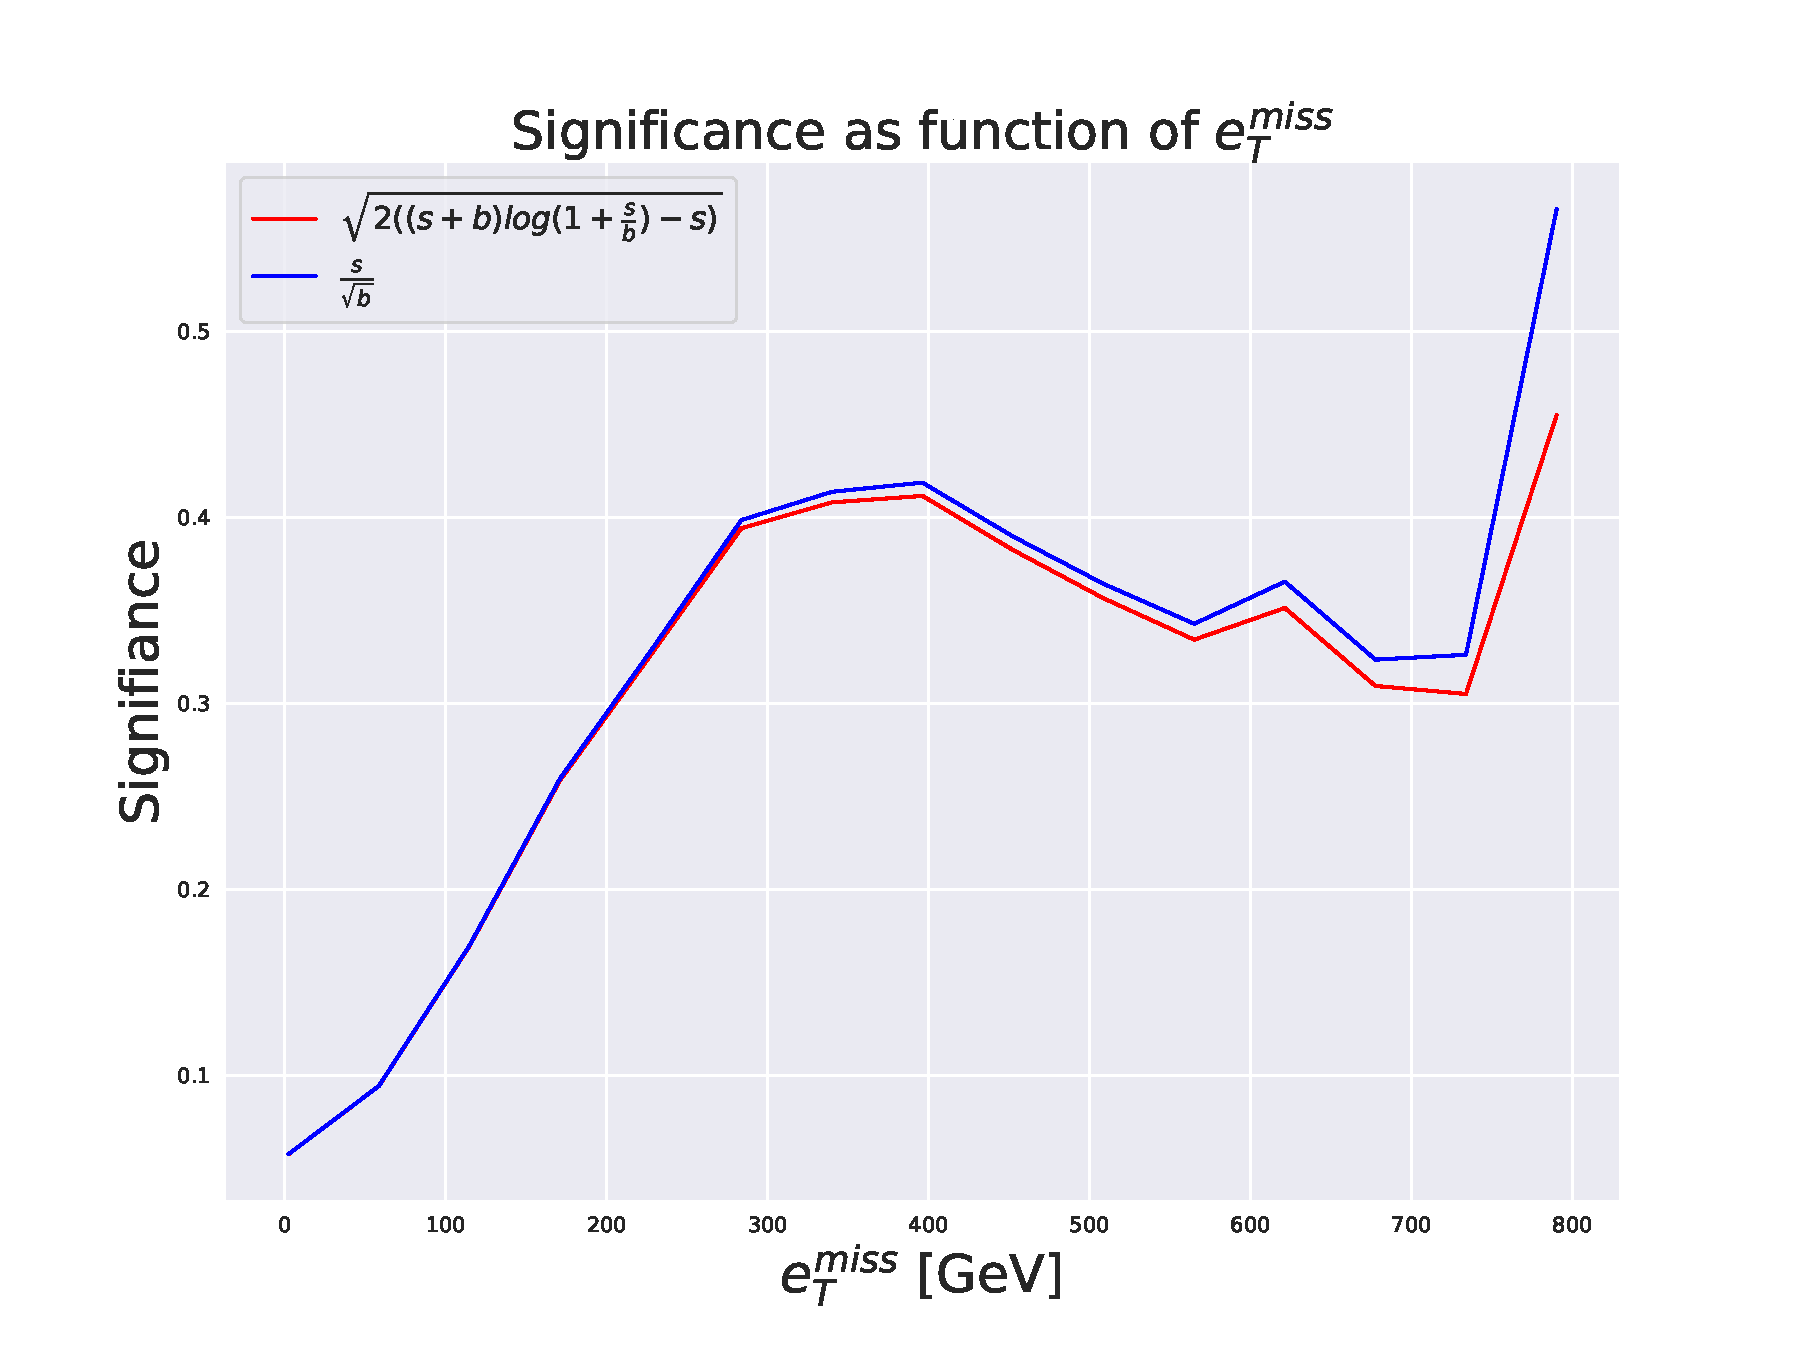
\includegraphics[width=\textwidth]{Figures/AE_testing/small/2lep/significance_etmiss_800p0p050_-1.6117055611472277.pdf}
        \caption{}
        \label{fig:AE_2lep_small_signi_800}
    \end{subfigure}
    \hfill      
    \caption[2lep shallow network | $800p50$ | AE]{Reconstruction error (a), $e_T^{miss}$ signal region (b) and significance as function of 
    $e_T^{miss}$ (c) for the shallow regular autoencoder using SUSY $800p50$. 
    (a) shows the reconstruction error distribution for the SM MC and the SUSY signal. 
    The autoencoder produces a slope-like shape that is highly shifted to the lower end of the reconstruction error range
for the background. The signal is more evenly spread out along the x-axis. The peaks of the two distributions are totally separated
with two orders of magnitude in reconstruction error. (b) shows the $e_T^{miss}$
T distribution for the SM MC and the SUSY signal in the signal region. The signal region is made using a cut around
$10^{-1.61}$. Most of the background is removed, and the peaks of the SM MC and signal distributions are
somewhat separated. (c) shows the significance as function of $e_T^{miss}$. The peak is put 
around a cut of about 400 GeV in the $e_T^{miss}$, with a significance of around $0.42$.}
    \label{fig:AE_2lep_small_rec_sig_signi_800}
\end{figure}


Figures \ref{fig:AE_2lep_big_rec_sig_signi_450}, \ref{fig:AE_2lep_small_rec_sig_signi_450}, 
\ref{fig:AE_2lep_big_rec_sig_signi_800} and \ref{fig:AE_2lep_small_rec_sig_signi_800} display three 
subplots each, containing the total reconstruction error distributions (a), the $e_T^{miss}$ signal regions (b), 
and the significance as function of a cut in $e_T^{miss}$ (c). 
By comparing the reconstruction error distributions of the AEs trained on the two lepton dataset 
(Figure \ref{fig:AE_2lep_big_450} - \ref{fig:AE_2lep_small_800}) with the corresponding figures from ones trained on the 3 lepton dataset 
(Figure \ref{fig:AE_3lep_big_450} - \ref{fig:AE_3lep_small_800}.) we see a clear tendency towards the signals having a larger reconstruction 
error compared with the SM MC. This indicates that as we increase the 
statistics, in other words the amount of background events 
used for training, the ability of the autoencoder to learn the internal structure increases. 
As expected, Z-boson production in association with jets along with $t\bar{t}$ are the channels with the highest statistics 
in the 2 lepton + $e_T^{miss}$ dataset, thus it should be easier to for the AEs to better reconstruct 
those events. However, note the amount of diboson in the higher end of the reconstruction error 
histograms, as well as in the $e_T^{miss}$ distribution after applying a cut on the reconstruction error.  \par
In figures \ref{fig:AE_2lep_big_etmiss_450}, \ref{fig:AE_2lep_small_etmiss_450}, \ref{fig:AE_2lep_big_etmiss_800} and  
\ref{fig:AE_2lep_small_etmiss_800} we have the $e_T^{miss}$ distributions for 
the least strict cuts for the regular autoencoder models. 
The corresponding significances obtained by applying a cut in the etmiss distribution of the most inclusive 
signal regions are shown in figures \ref{fig:AE_2lep_big_signi_450}, \ref{fig:AE_2lep_small_signi_450}, \ref{fig:AE_2lep_big_signi_800} 
and  \ref{fig:AE_2lep_small_signi_800}. The highest significance (of about 1.75) was found with the shallow autoencoder 
with the SUSY $450p300$ signal model. It should be noted that the significance 
for the $800p50$ signal model is a lot smaller than for the $450p300$ signal model, even though the separation 
shown in figures \ref{fig:AE_2lep_big_450}, \ref{fig:AE_2lep_small_450}, \ref{fig:AE_2lep_big_800}, 
\ref{fig:AE_2lep_small_800} would suggest otherwise. 
In order to better understand the performance of the AEs a comparison of the maximum significance obtained from a 
cut in etmiss before and after imposing a requirement on the reconstruction error was performed. Before any cut 
in reconstruction error the maximum significances obtained were 0.017 and 0.0014 for the $450p300$ and $800p50$ 
points, respectively. This can be compared with the significances of 2.4 and 0.42 obtained after the cut in 
reconstruction error. Note that for the results without the reconstruction error cut no other cuts were 
applied to enhance the signal over background ratio and thus a better significance would be expected in a 
more comprehensive analysis.

\par

\subsubsection*{Variational autoencoder performance}

\begin{figure}[h!]
    \centering
    \begin{subfigure}{.49\textwidth}
        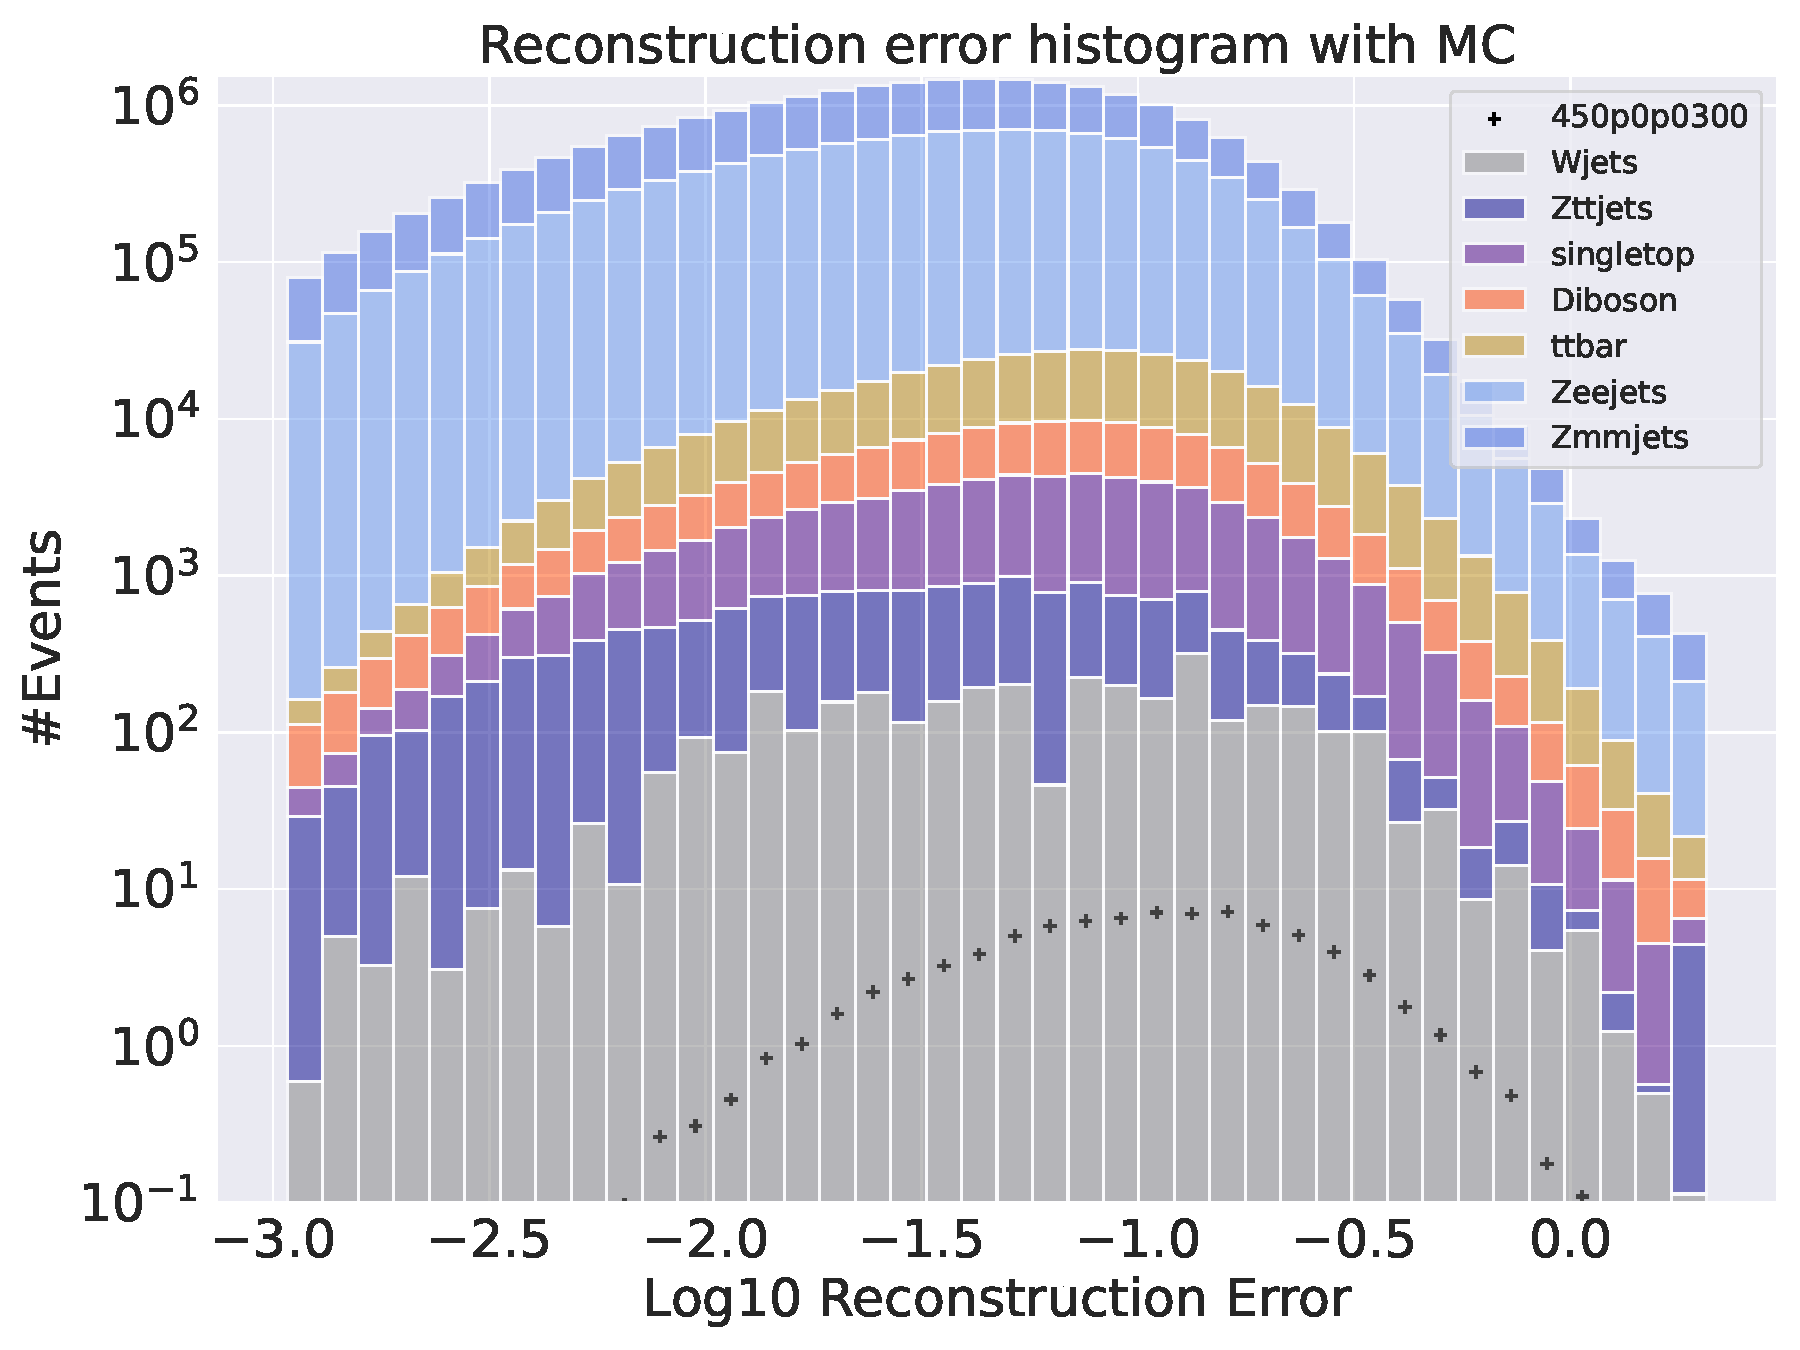
\includegraphics[width=\textwidth]{Figures/VAE_testing/small/2lep/b_data_recon_big_rm3_feats_sig_450p0p0300_.pdf}
        \caption{ }
        \label{fig:VAE_2lep_big_450}
    \end{subfigure}
    \hfill
    \begin{subfigure}{.49\textwidth}
        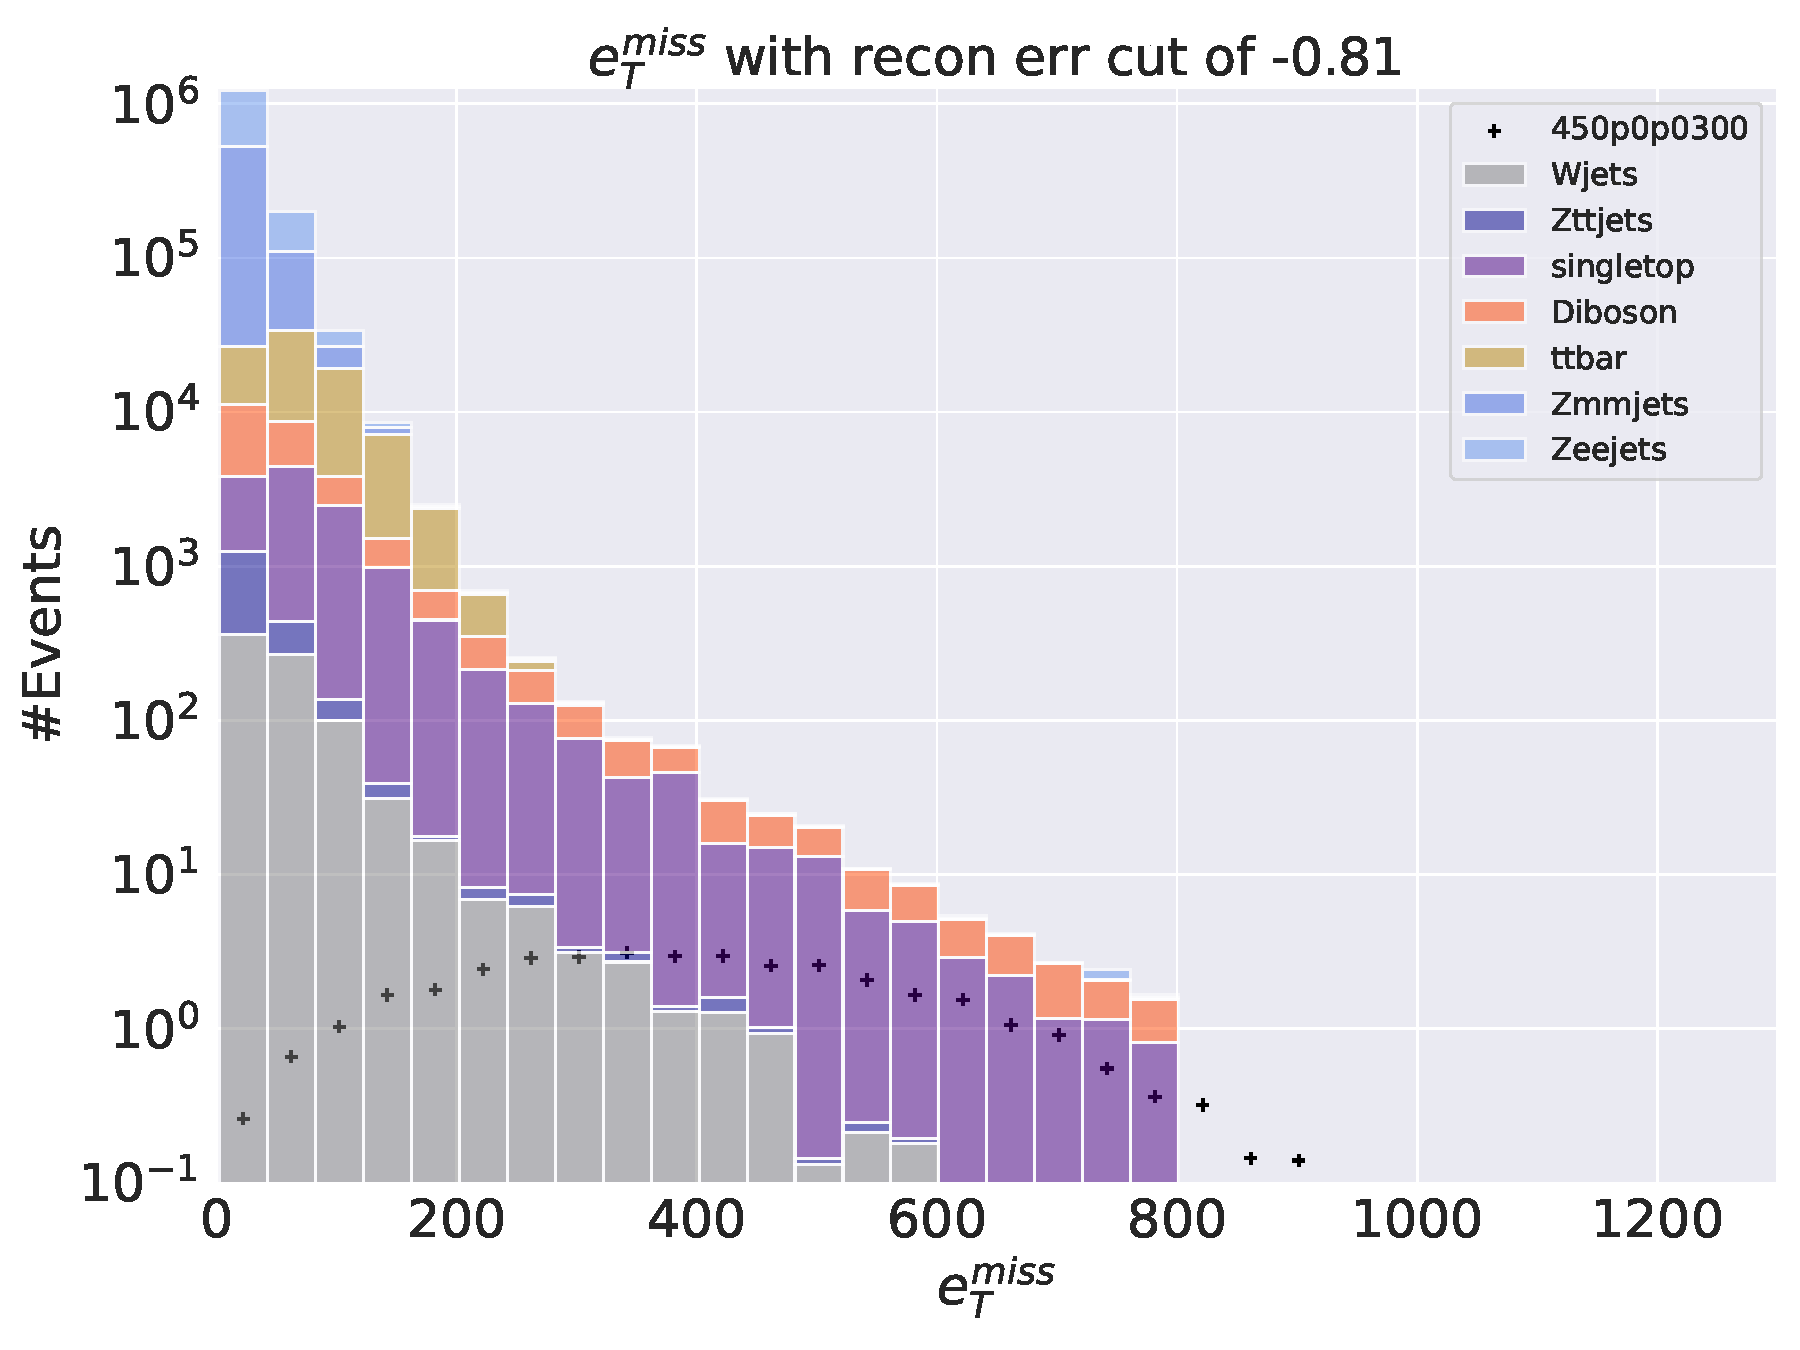
\includegraphics[width=\textwidth]{Figures/VAE_testing/big/2lep/b_data_recon_big_rm3_feats_sig_450p0p0300_recon_errcut_-0.81.pdf}
        \caption{}
        \label{fig:VAE_2lep_big_etmiss_450}
    \end{subfigure}
    \hfill 
    \begin{subfigure}{.49\textwidth}
        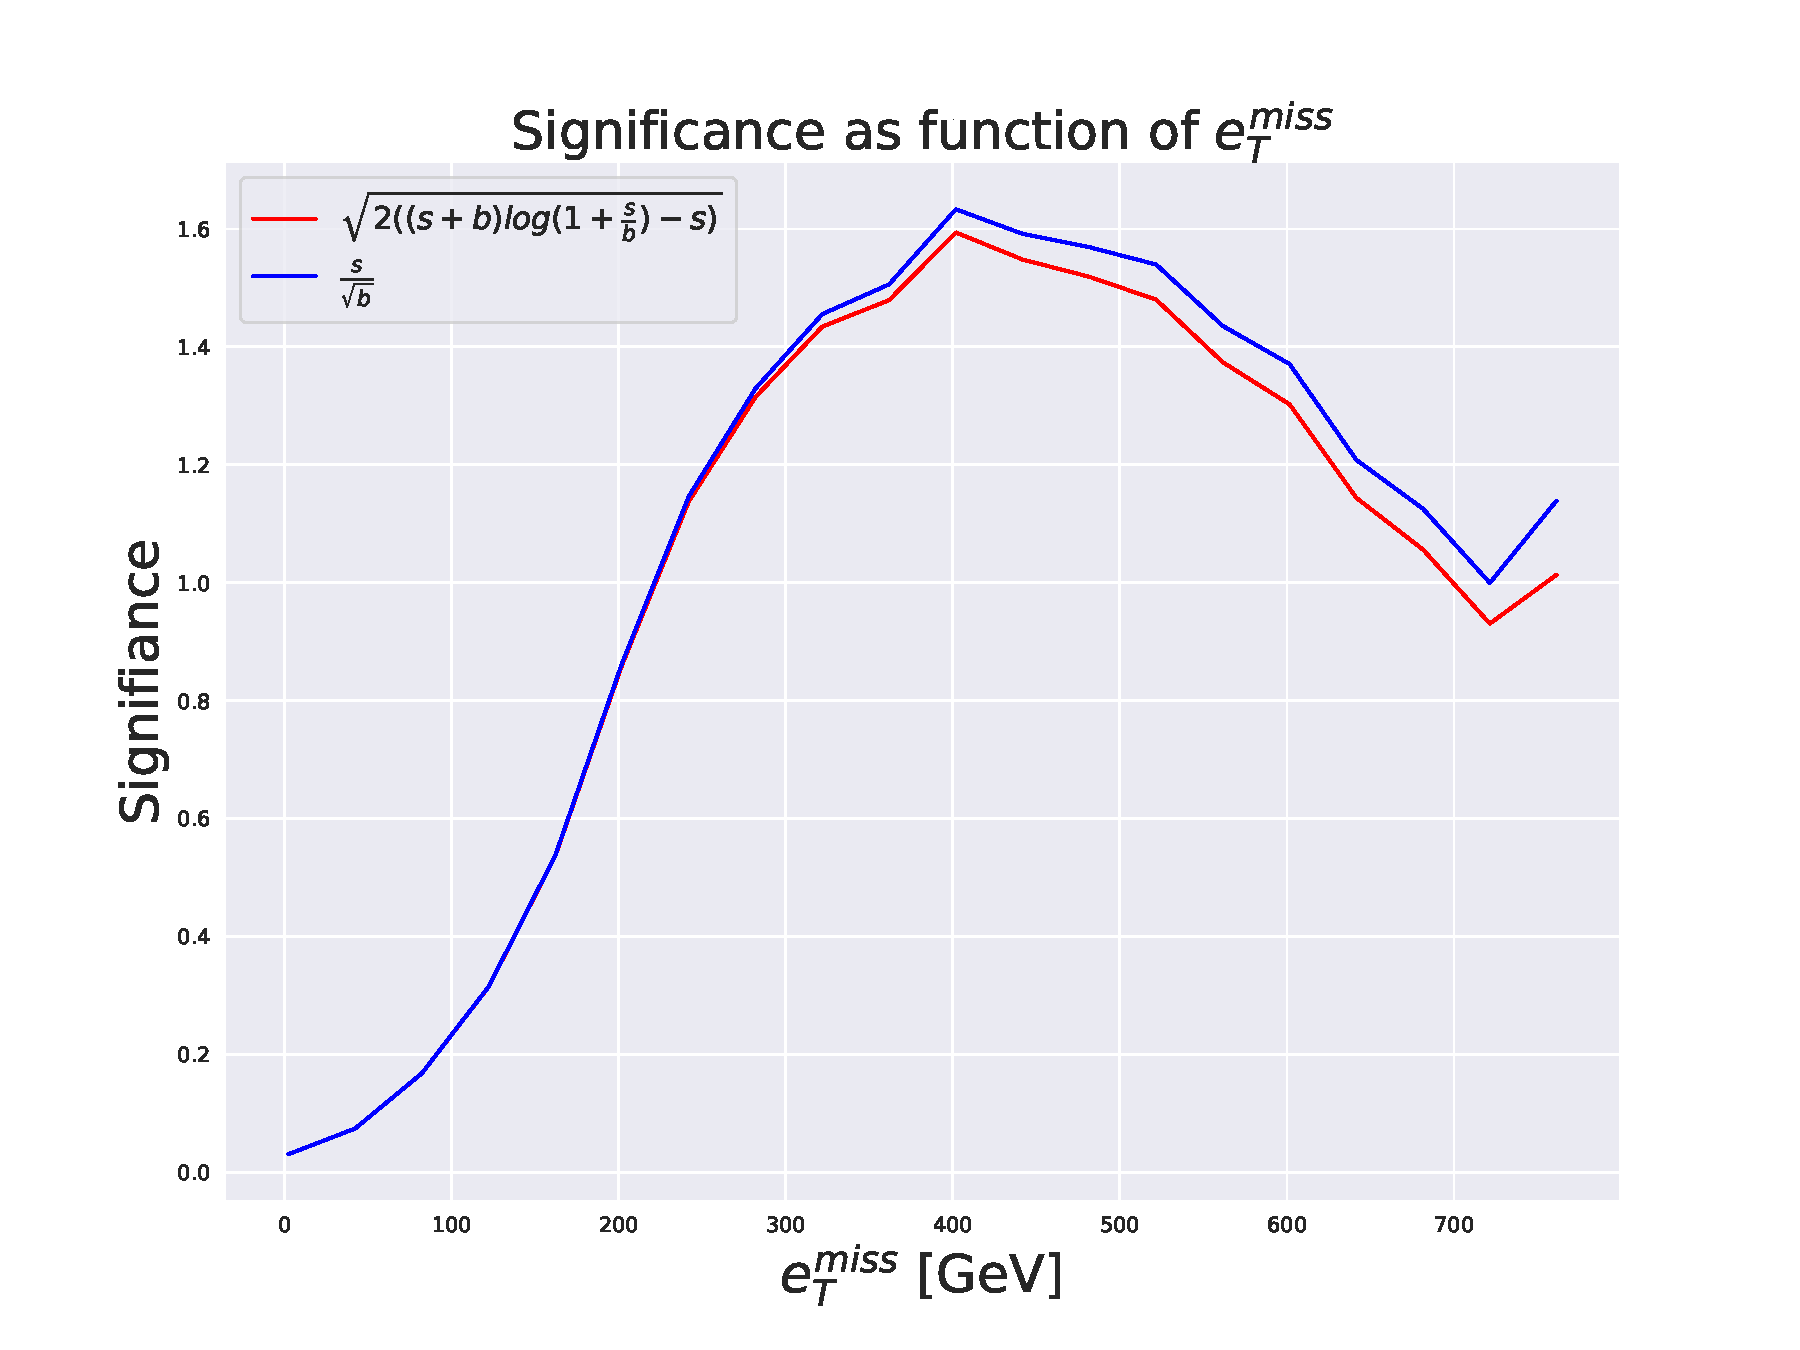
\includegraphics[width=\textwidth]{Figures/VAE_testing/big/2lep/significance_etmiss_450p0p0300_-0.8121874101107931.pdf}
        \caption{}
        \label{fig:VAE_2lep_big_signi_450}
    \end{subfigure}
    \hfill      
    \caption[2lep deep network | $450p300$ | VAE]{Reconstruction error (a), $e_T^{miss}$ signal region (b) and significance as function of 
    $e_T^{miss}$ (c) for the deep variational autoencoder using SUSY $450p300$. 
    (a) shows that the peak of the distribution is somewhat centered in the middle 
    of the reconstruction error range forming a hill-like shape. The peaks of the background and signal 
    distributions are not well separated, with almost identical reconstruction error pattern. (b) 
    shows a signal region with large background distribution. The signal region is made using a cut around
    $10^{-0.81}$. The peaks in the signal region are also somewhat 
    separated, but the overall distributions are overlapping still. 
    (c) shows the significance as function of $e_T^{miss}$. 
    The peak significance is around 1.61 at around 400 GeV.}
    \label{fig:VAE_2lep_big_rec_sig_signi_450}
\end{figure}

\begin{figure}[h!]
    \centering
    \begin{subfigure}{.49\textwidth}
        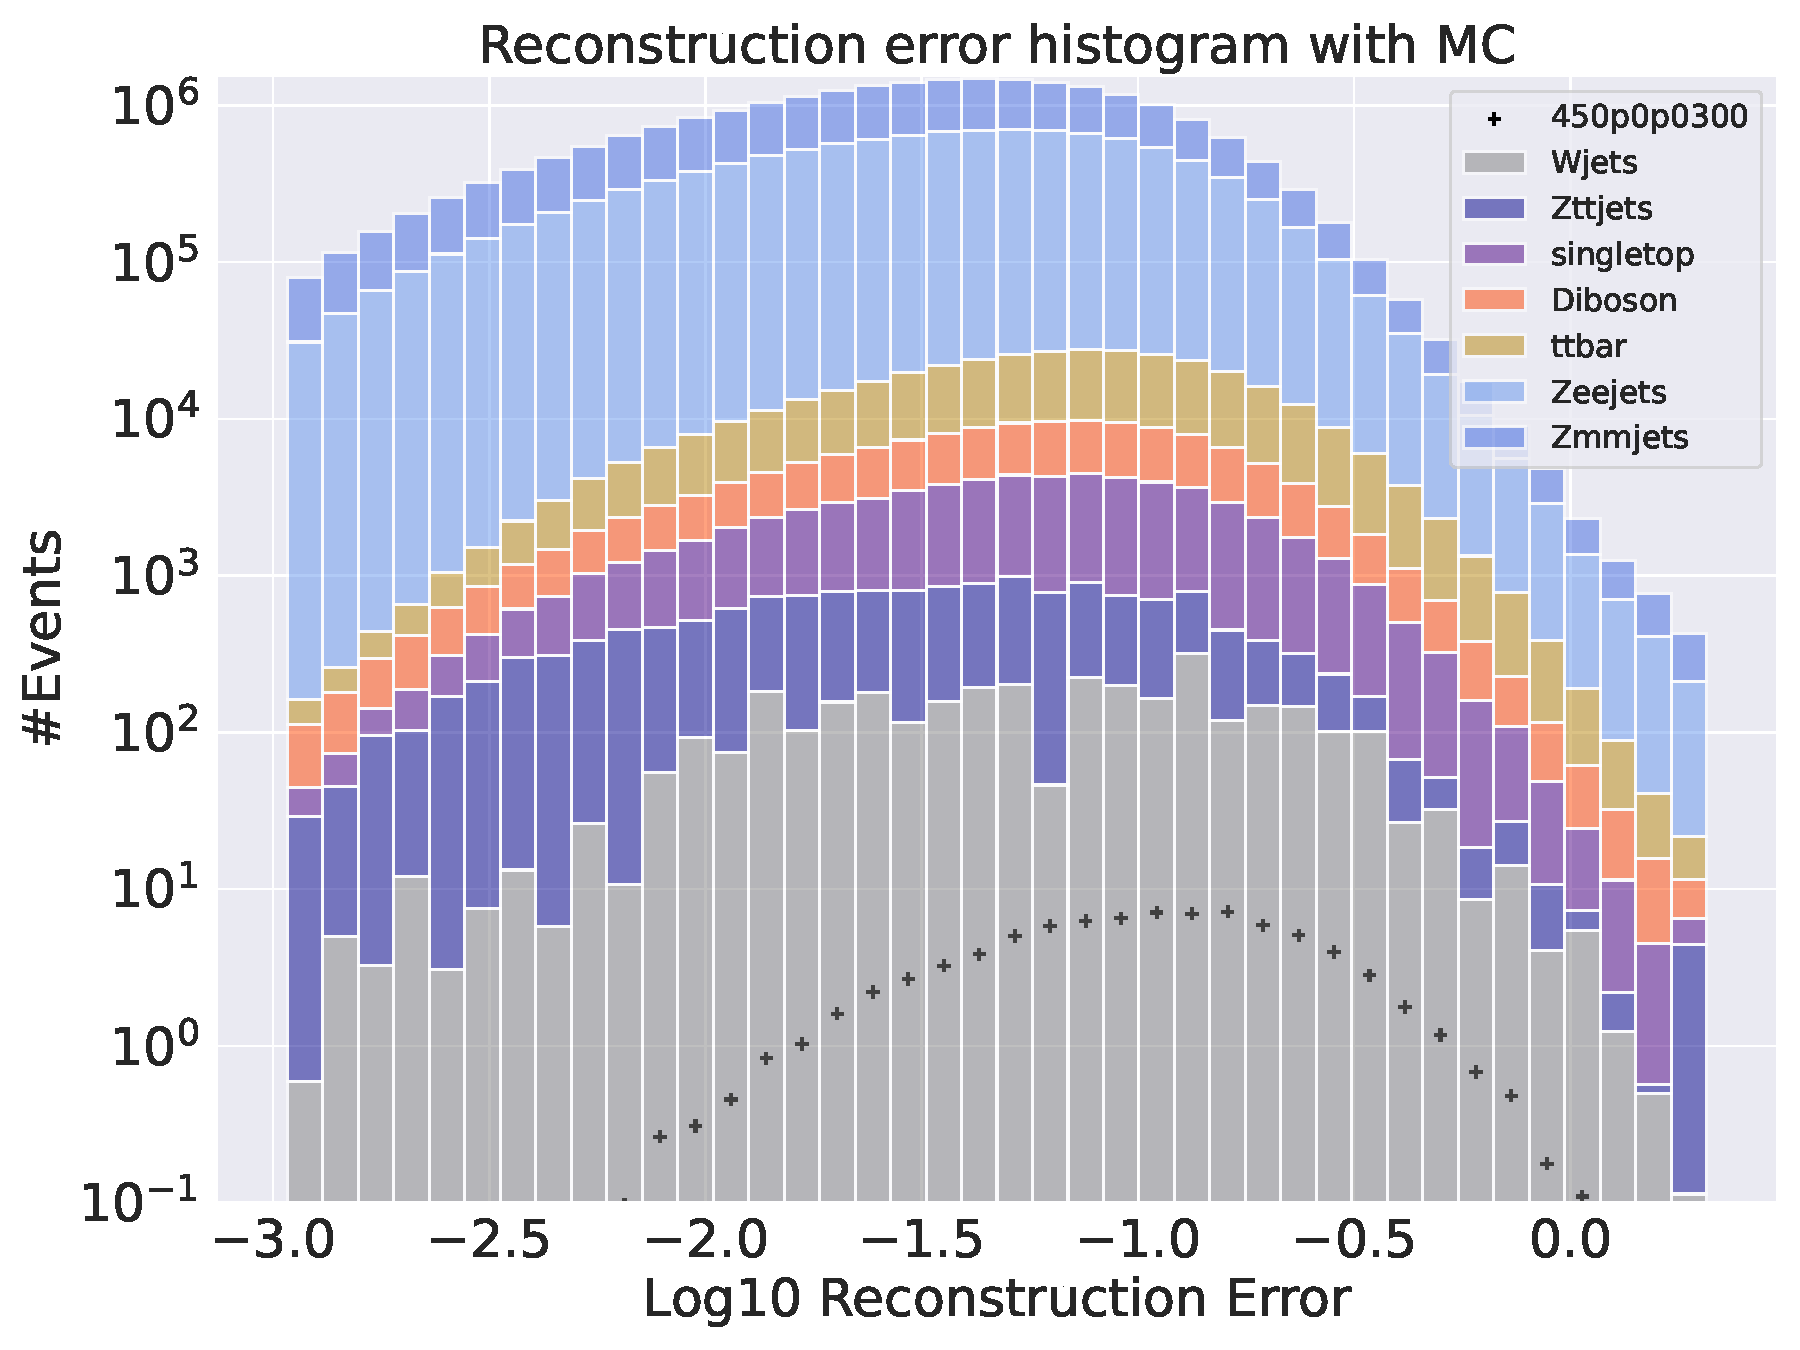
\includegraphics[width=\textwidth]{Figures/VAE_testing/small/2lep/b_data_recon_big_rm3_feats_sig_450p0p0300_.pdf}
        \caption{ }
        \label{fig:VAE_2lep_small_450}
    \end{subfigure}
    \hfill
    \begin{subfigure}{.49\textwidth}
        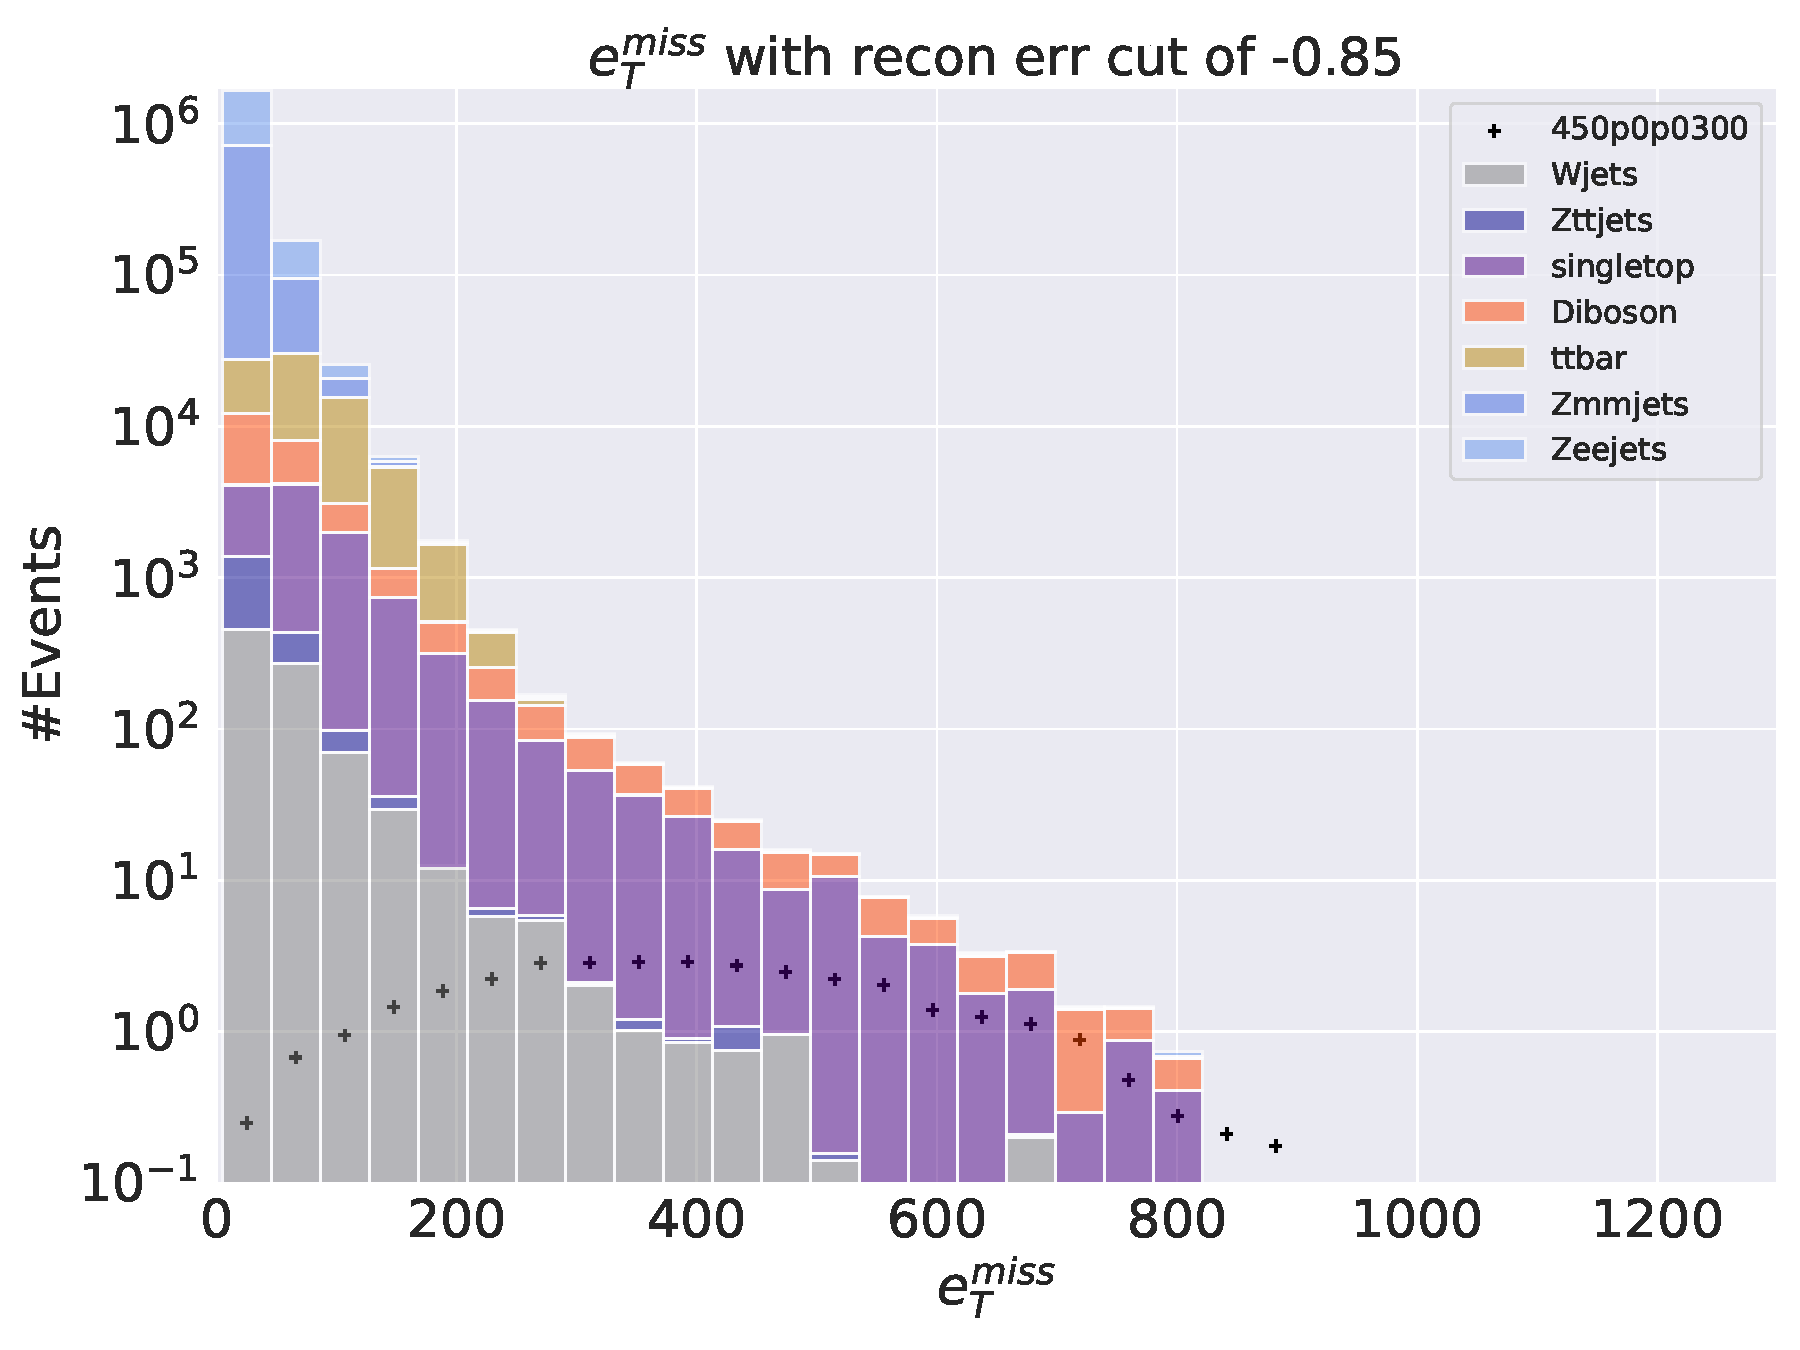
\includegraphics[width=\textwidth]{Figures/VAE_testing/small/2lep/b_data_recon_big_rm3_feats_sig_450p0p0300_recon_errcut_-0.85.pdf}
        \caption{}
        \label{fig:VAE_2lep_small_etmiss_450}
    \end{subfigure}
    \hfill  
    \begin{subfigure}{.49\textwidth}
        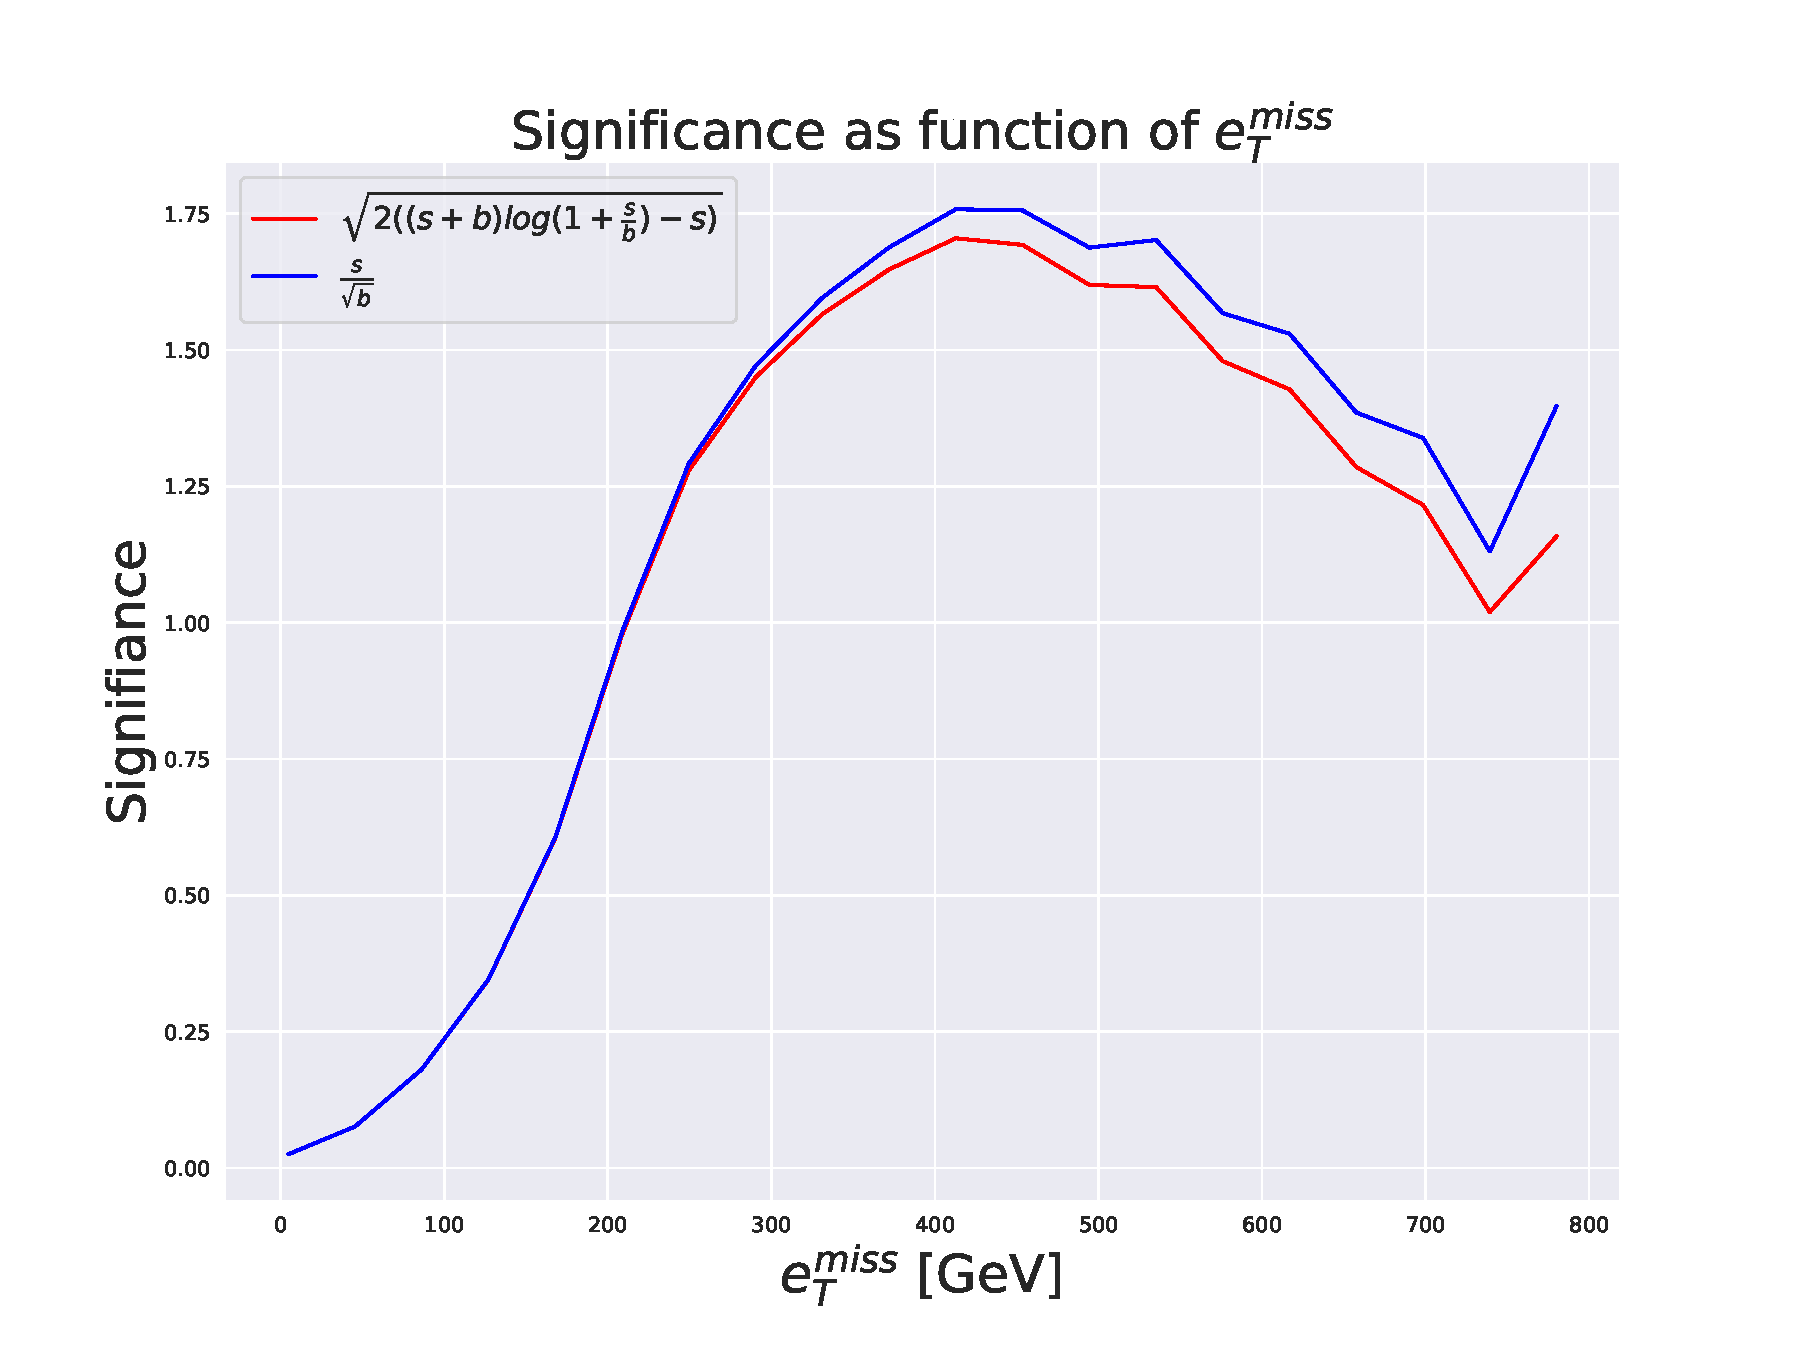
\includegraphics[width=\textwidth]{Figures/VAE_testing/small/2lep/significance_etmiss_450p0p0300_-0.8484803499636524.pdf}
        \caption{}
        \label{fig:VAE_2lep_small_signi_450}
    \end{subfigure}
    \hfill      
    \caption[2lep shallow network | $450p300$ | VAE]{Reconstruction error (a), $e_T^{miss}$ signal region (b) and significance as function of 
    $e_T^{miss}$ (c) for the shallow variational autoencoder using SUSY $450p300$.
    (a) shows that the peak of the distribution is somewhat centered in the middle 
    of the reconstruction error range forming a hill-like shape. The peaks of the background and signal 
    distributions are not well separated, with almost identical reconstruction error pattern. (b) 
    shows a signal region with large background distribution. The signal region is made using a cut around
    $10^{-0.85}$. The peaks in the signal region are also somewhat 
    separated, but the overall distributions are overlapping still. 
    (c) shows the significance as function of $e_T^{miss}$. 
The peak significance is around 1.75 at around 420-450 GeV.}
    \label{fig:VAE_2lep_small_rec_sig_signi_450}
\end{figure}


\begin{figure}[h!]
    \centering
    \begin{subfigure}{.49\textwidth}
        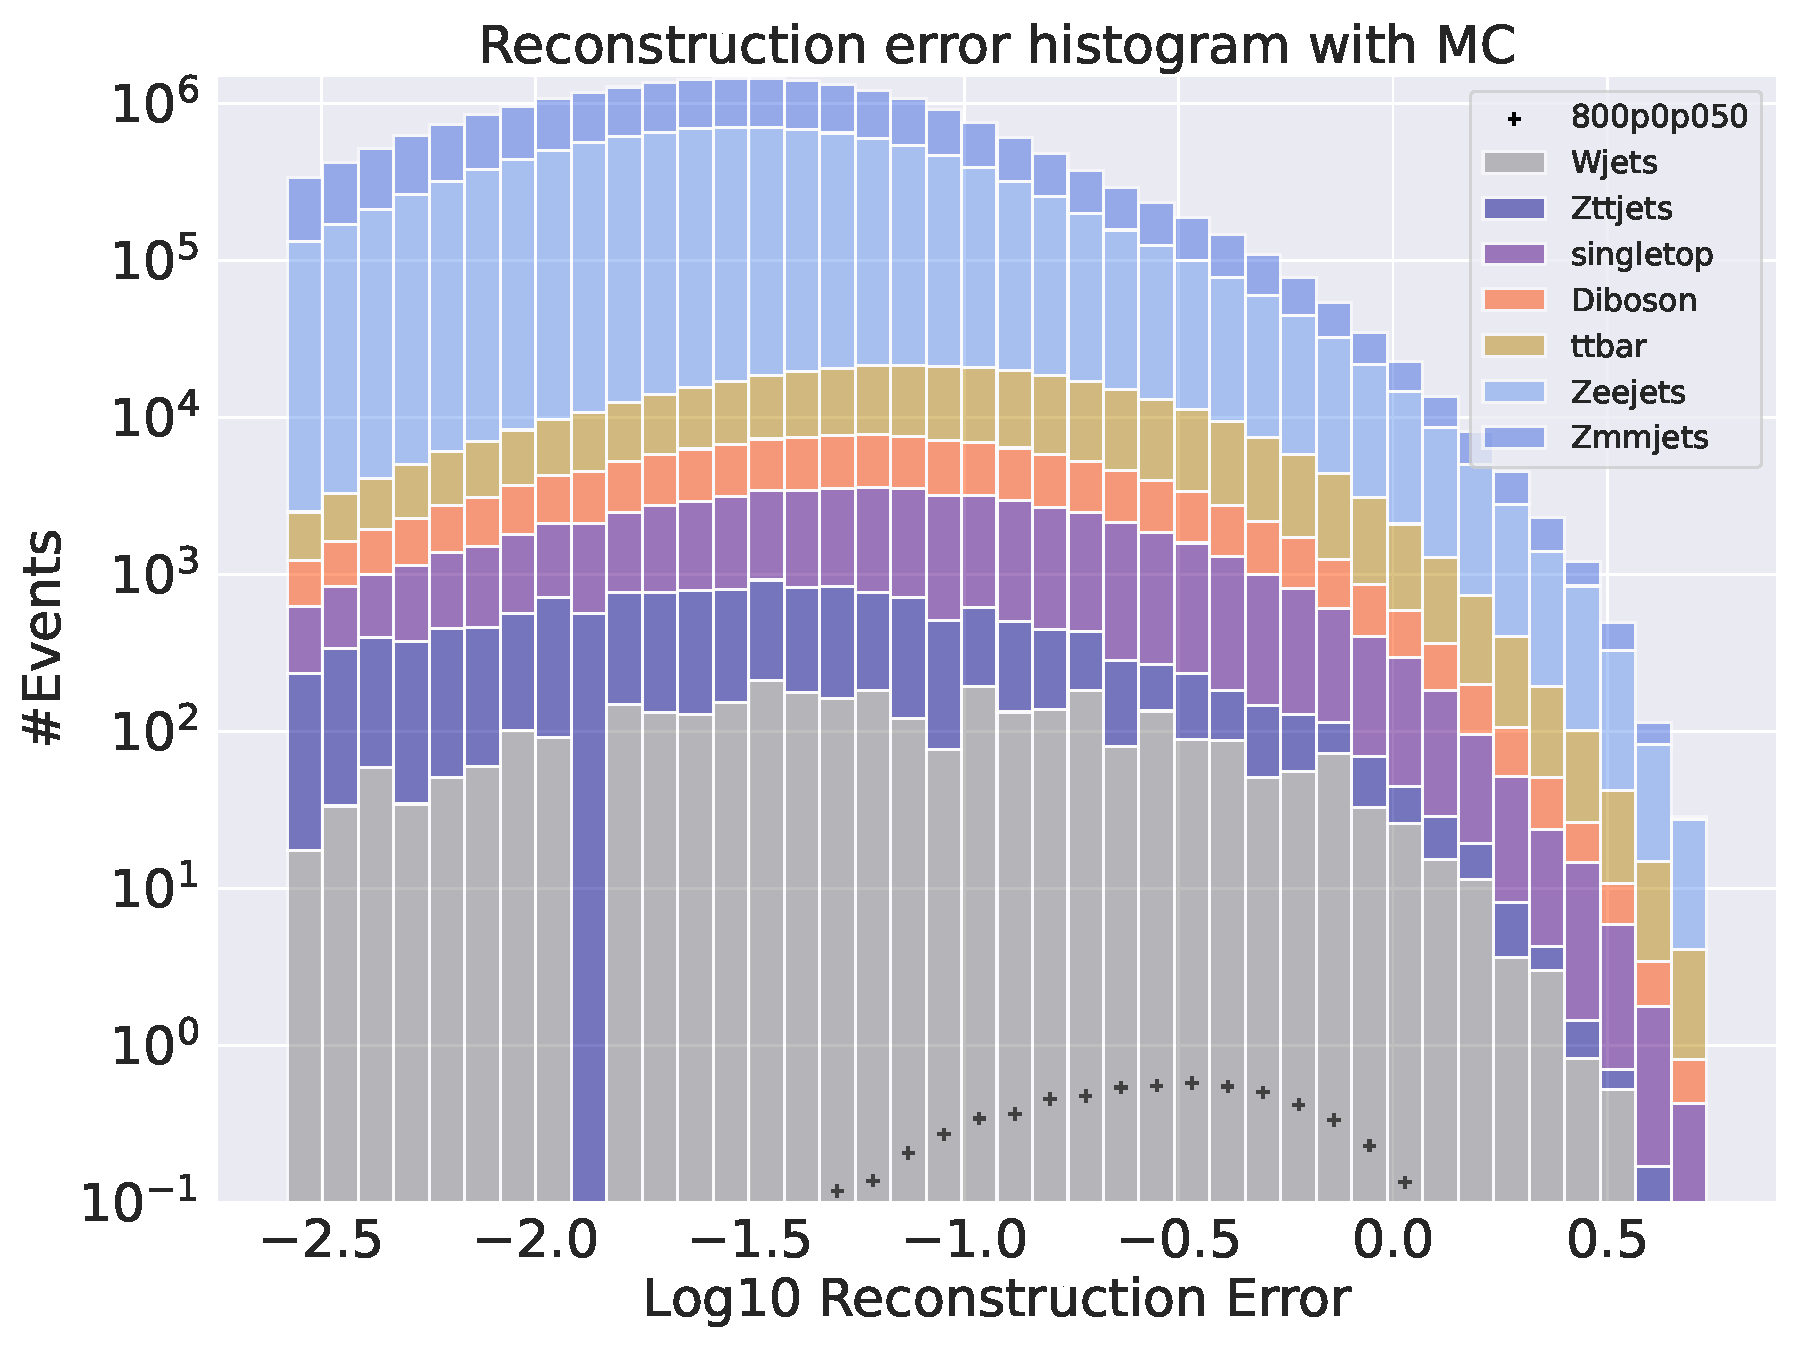
\includegraphics[width=\textwidth]{Figures/VAE_testing/big/2lep/b_data_recon_big_rm3_feats_sig_800p0p050_.pdf}
        \caption{ }
        \label{fig:VAE_2lep_big_800}
    \end{subfigure}
    \hfill
    \begin{subfigure}{.49\textwidth}
        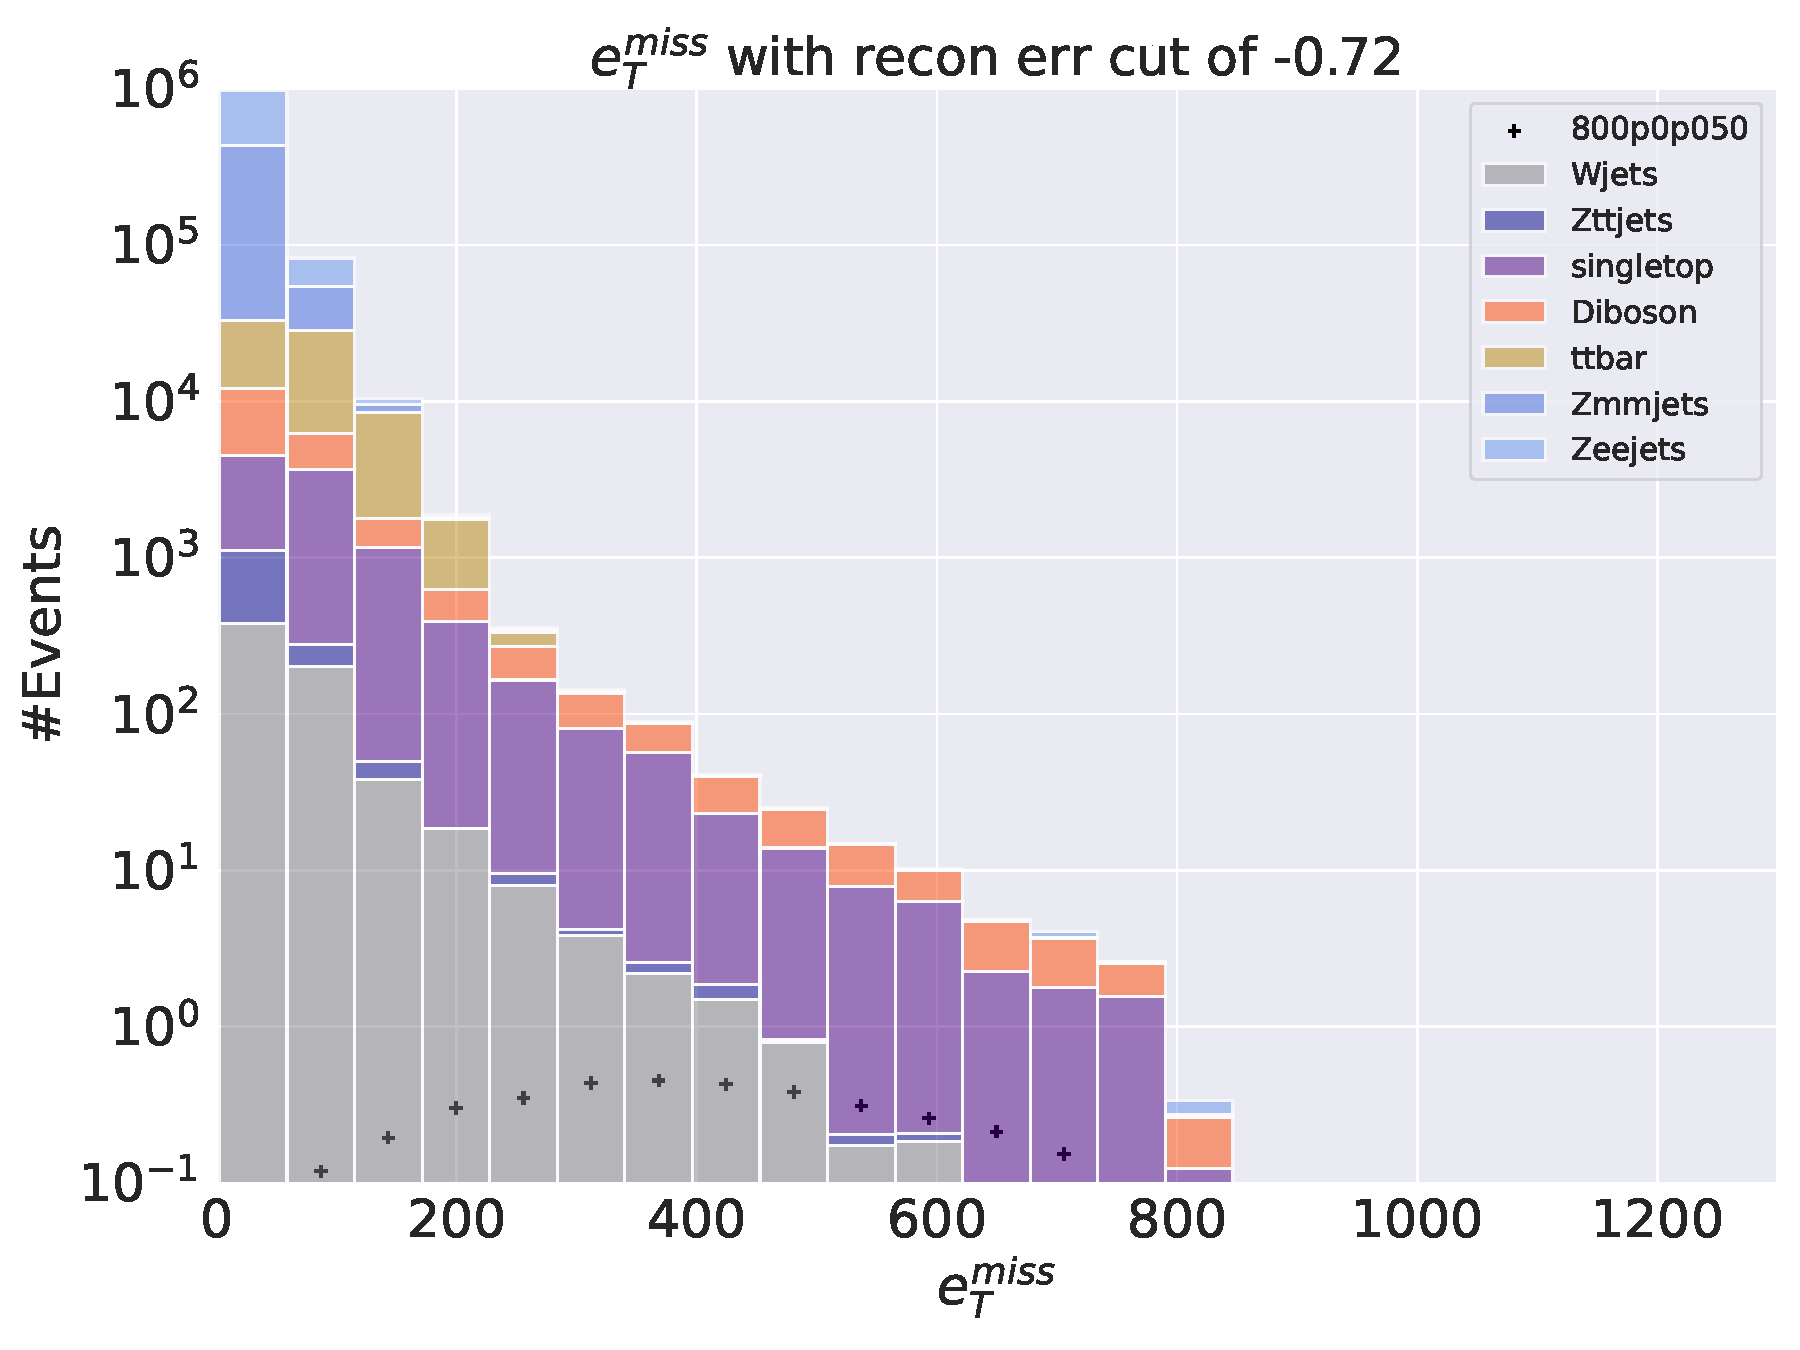
\includegraphics[width=\textwidth]{Figures/VAE_testing/big/2lep/b_data_recon_big_rm3_feats_sig_800p0p050_recon_errcut_-0.72.pdf}
        \caption{}
        \label{fig:VAE_2lep_big_etmiss_800}
    \end{subfigure}
    \hfill
      
    \begin{subfigure}{.49\textwidth}
        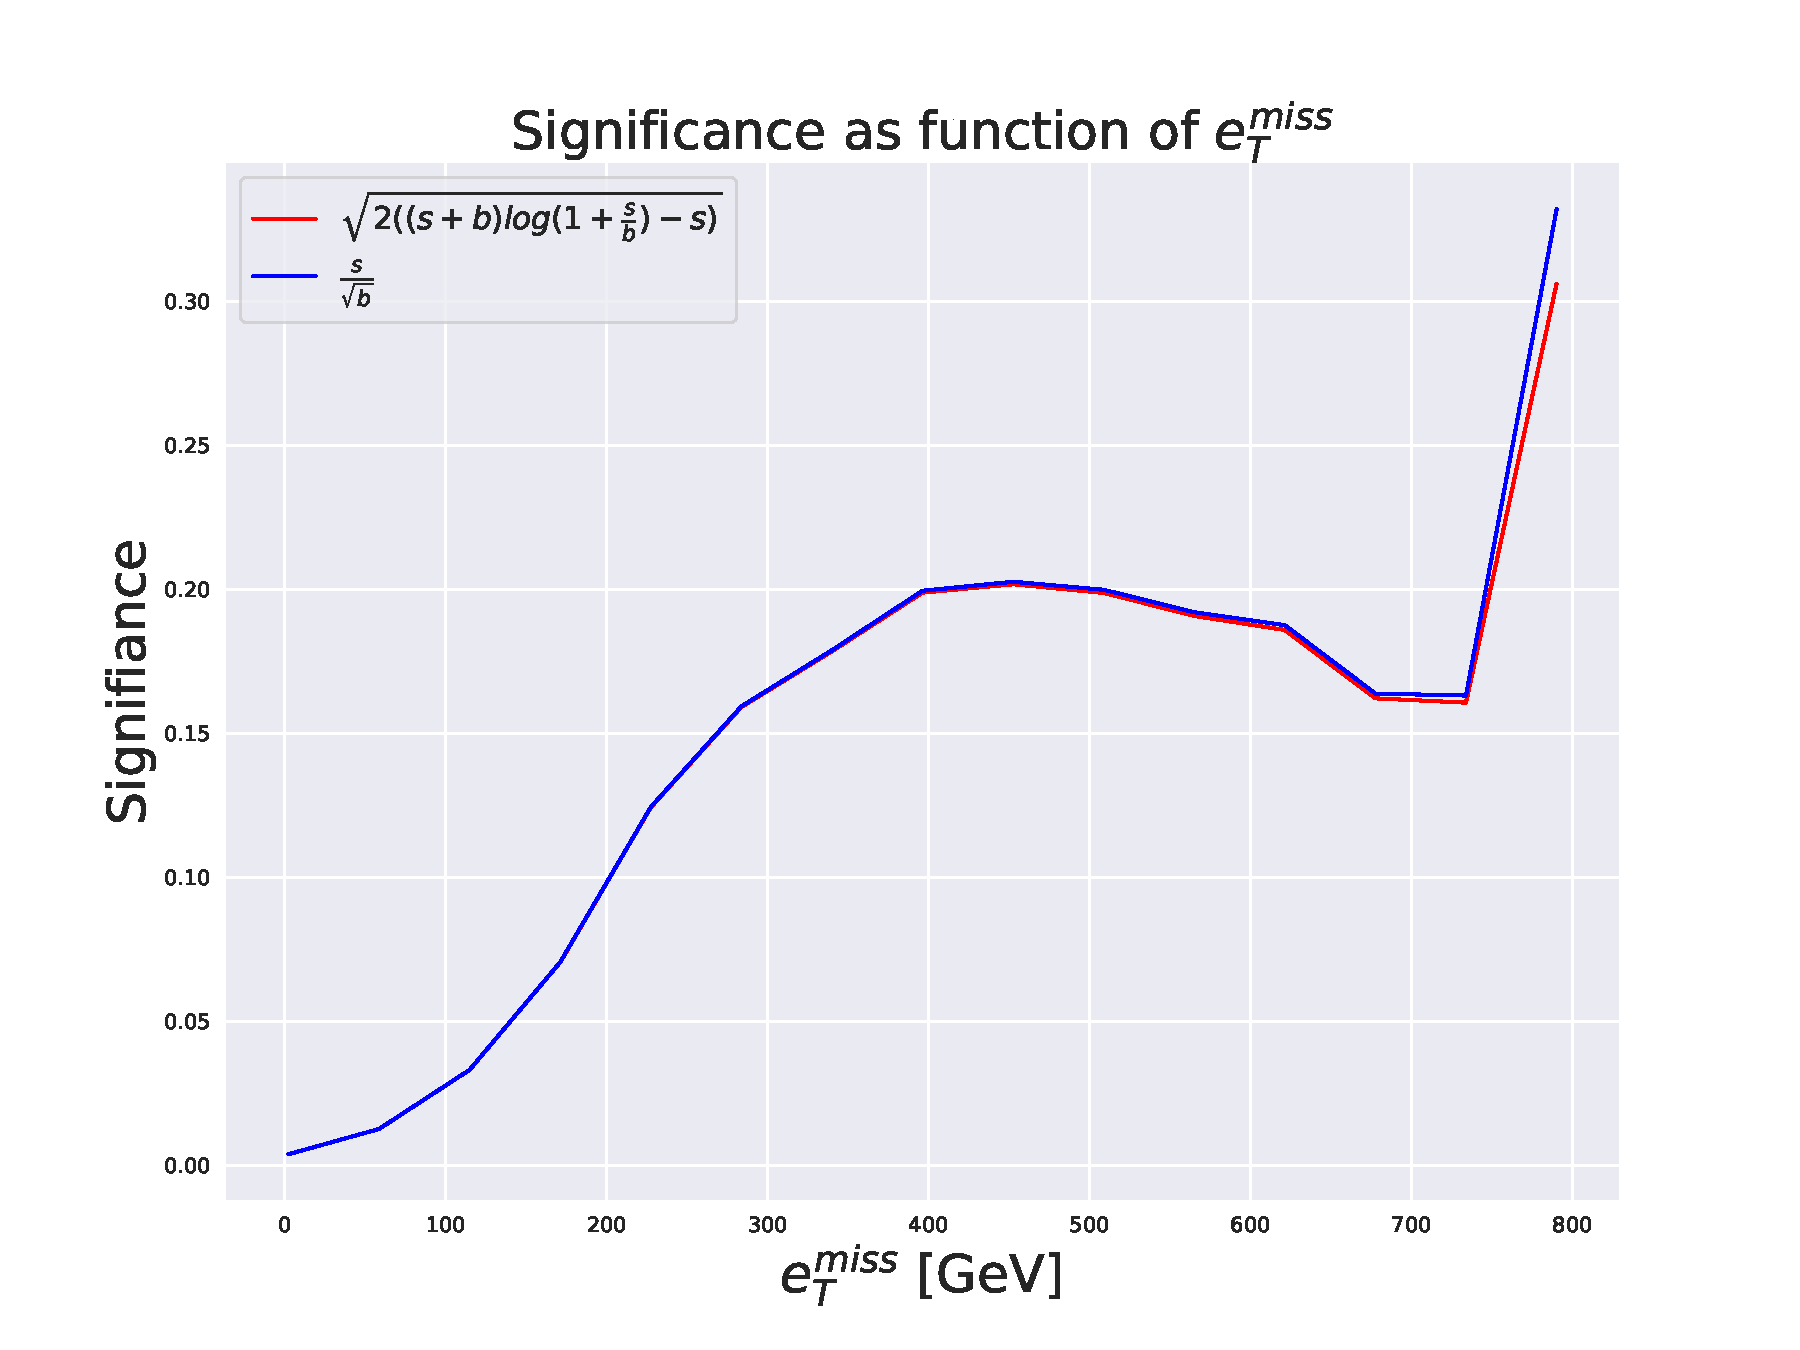
\includegraphics[width=\textwidth]{Figures/VAE_testing/big/2lep/significance_etmiss_800p0p050_-0.7232197345309495.pdf}
        \caption{}
        \label{fig:VAE_2lep_big_signi_800}
    \end{subfigure}
    \hfill      
    \caption[2lep deep network | $800p50$ | VAE]{Reconstruction error (a), $e_T^{miss}$ signal region (b) and significance as function of 
    $e_T^{miss}$ (c) for the deep variational autoencoder using SUSY $800p50$.
    (a) shows that the peak of the distribution is somewhat centered in the middle 
    of the reconstruction error range forming a hill-like shape. The peaks of the background and signal 
    distributions are not well separated, with some separation of distribution peaks. (b) 
    shows a signal region with large background distribution. The signal region is made using a cut around
    $10^{-0.72}$. The peaks in the signal region are also somewhat 
    separated, but the overall distributions are overlapping still. 
    (c) shows the significance as function of $e_T^{miss}$.
The peak significance is around 0.20 at around 450 GeV.}
    \label{fig:VAE_2lep_big_rec_sig_signi_800}
\end{figure}

\begin{figure}[h!]
    \centering
    \begin{subfigure}{.49\textwidth}
        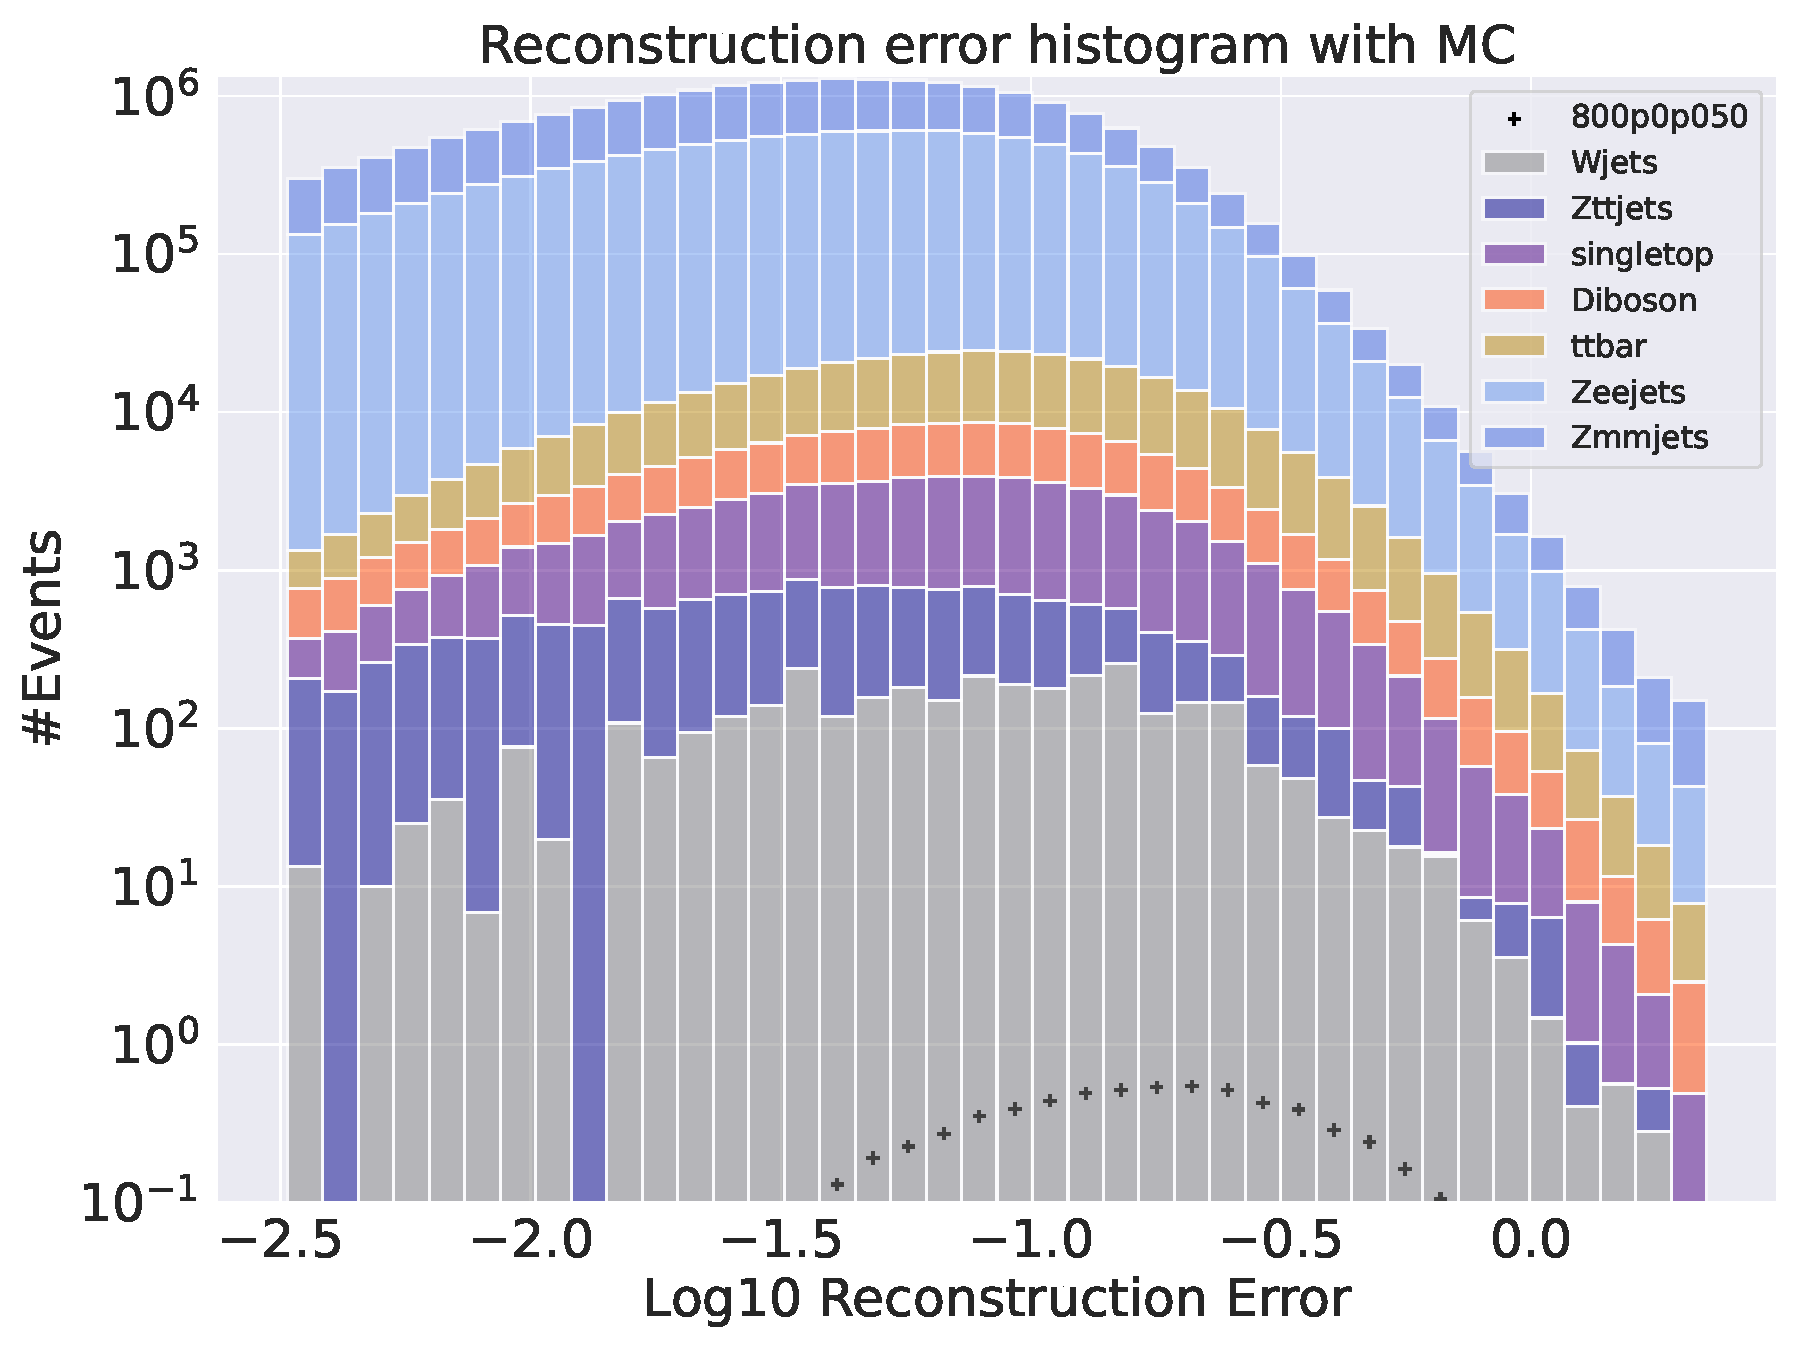
\includegraphics[width=\textwidth]{Figures/VAE_testing/small/2lep/b_data_recon_big_rm3_feats_sig_800p0p050_.pdf}
        \caption{ }
        \label{fig:VAE_2lep_small_800}
    \end{subfigure}
    \hfill
    \begin{subfigure}{.49\textwidth}
        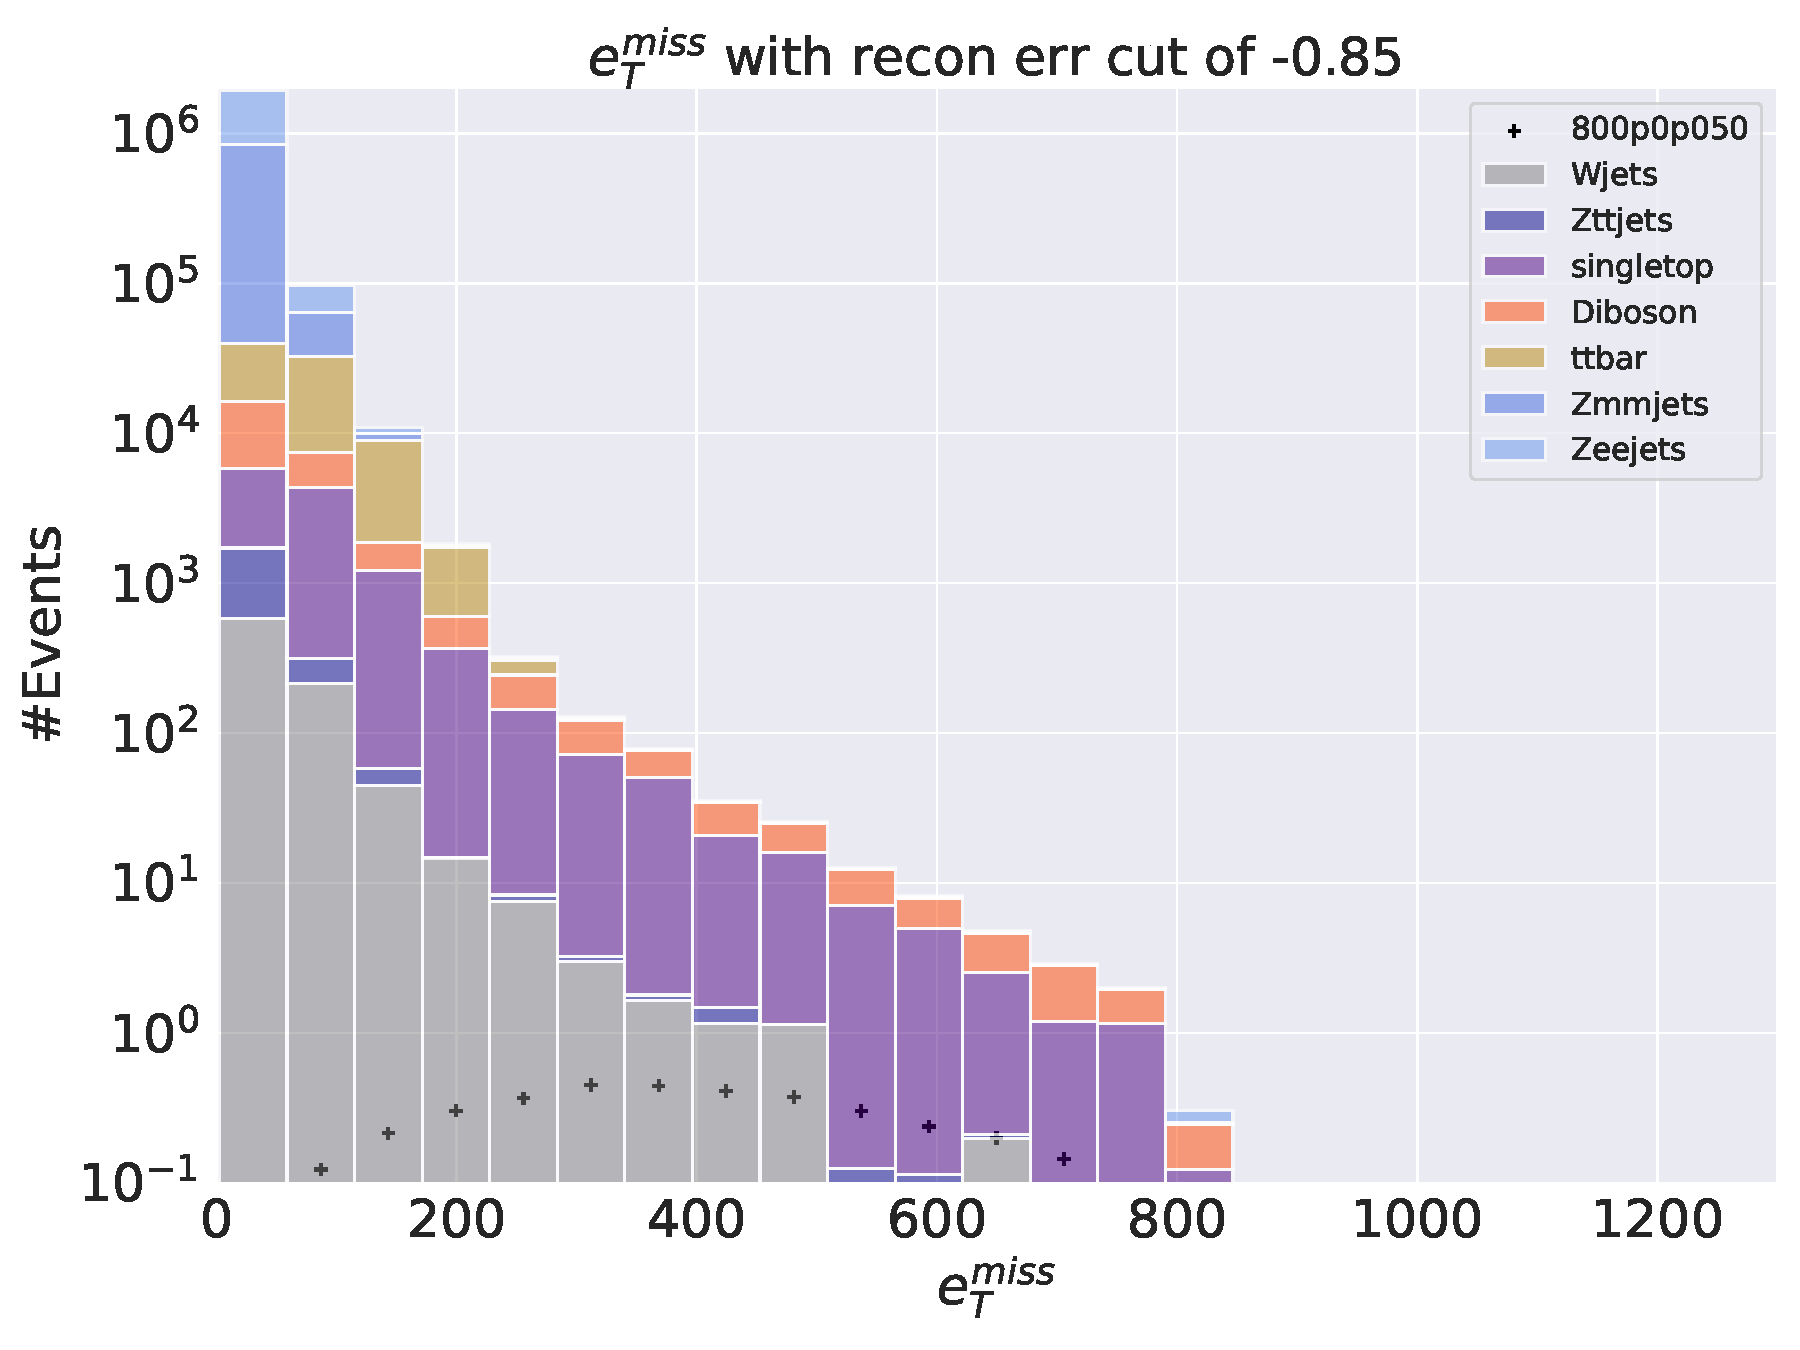
\includegraphics[width=\textwidth]{Figures/VAE_testing/small/2lep/b_data_recon_big_rm3_feats_sig_800p0p050_recon_errcut_-0.85.pdf}
        \caption{}
        \label{fig:VAE_2lep_small_etmiss_800}
    \end{subfigure}
    \hfill  
    \begin{subfigure}{.49\textwidth}
        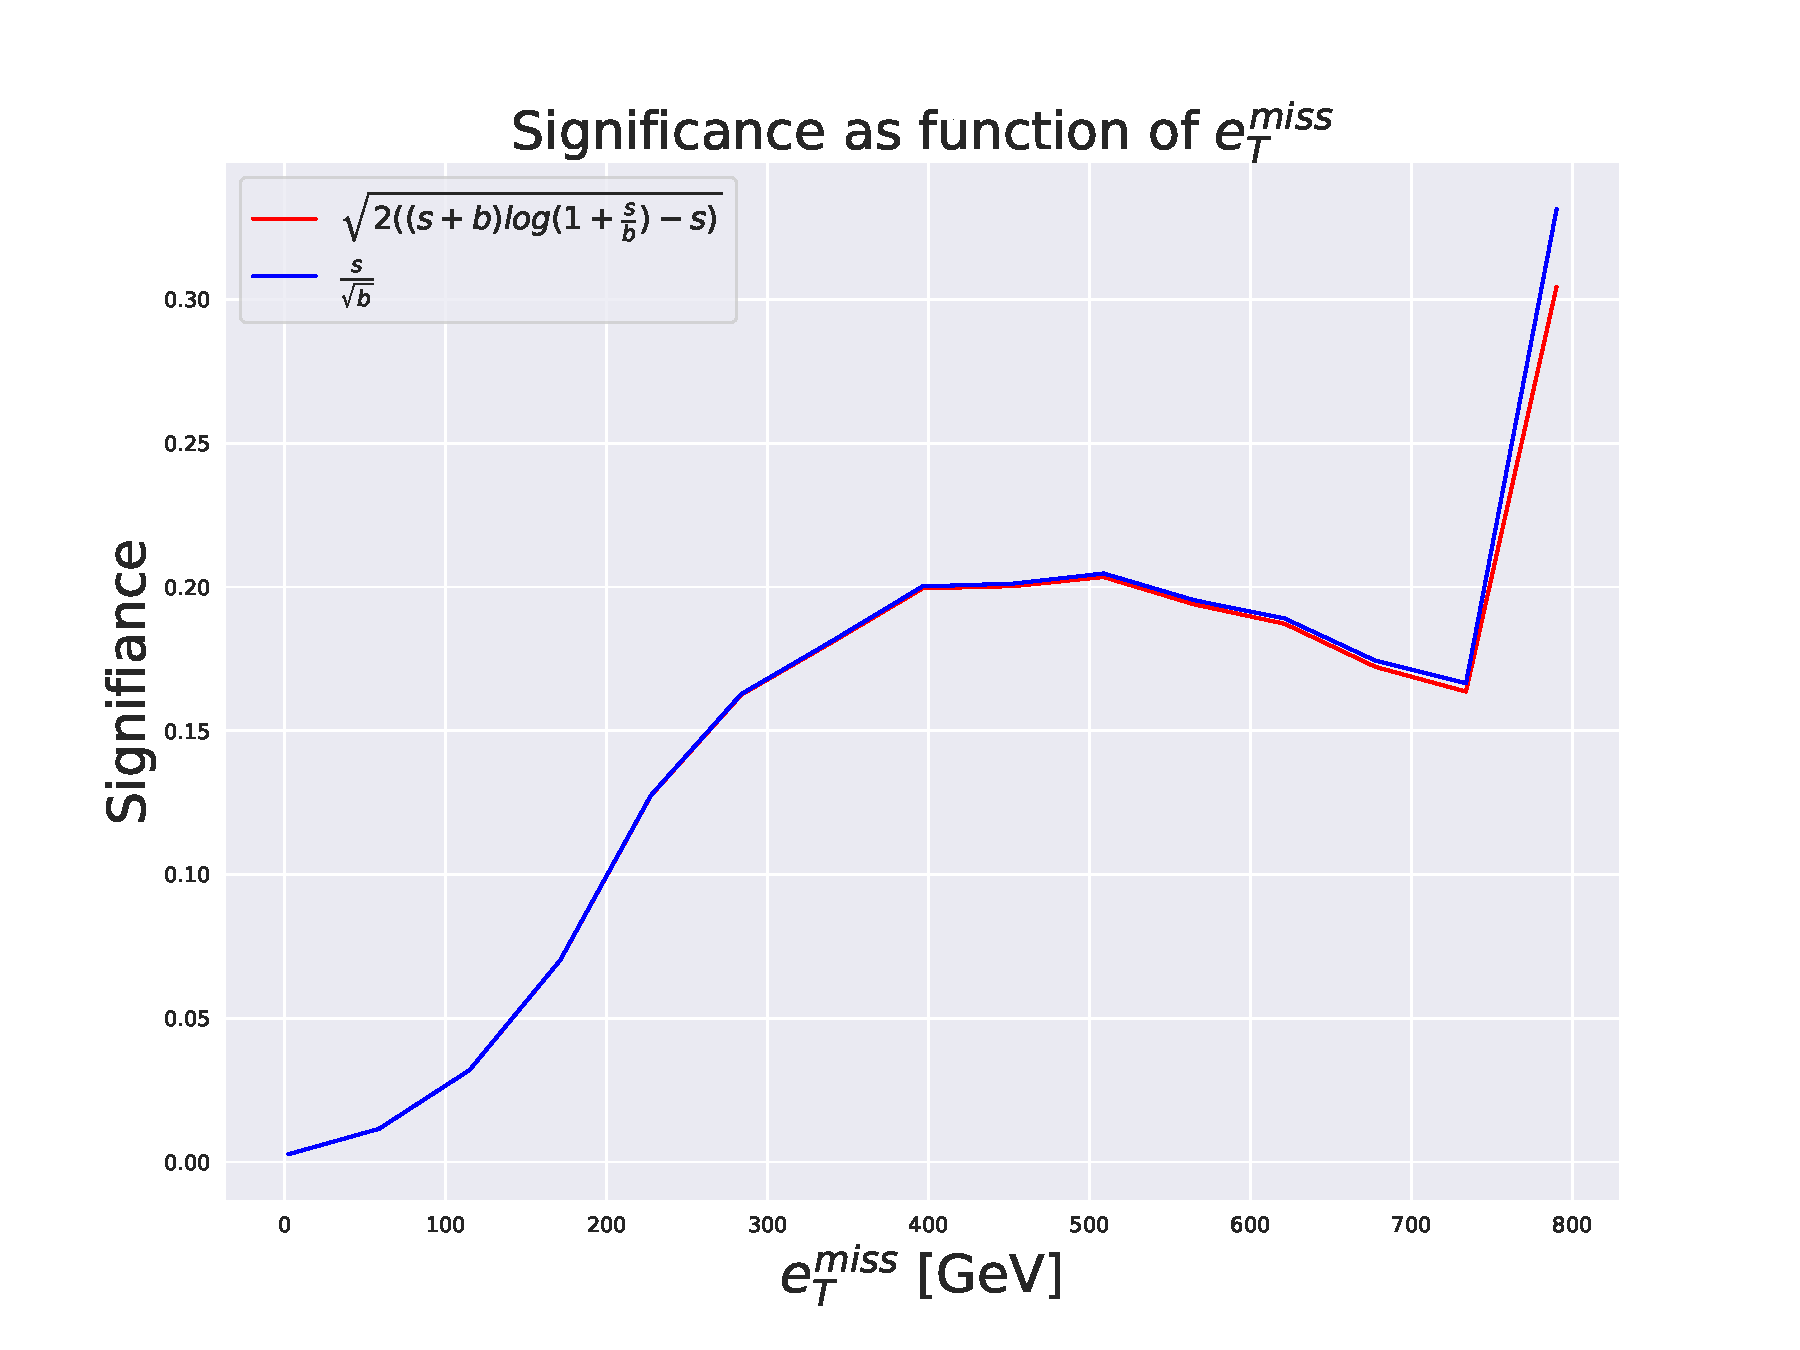
\includegraphics[width=\textwidth]{Figures/VAE_testing/small/2lep/significance_etmiss_800p0p050_-0.8542149600758421.pdf}
        \caption{}
        \label{ffig:VAE_2lep_small_signi_800}
    \end{subfigure}
    \hfill      
    \caption[2lep shallow network | $800p50$ | VAE]{Reconstruction error (a), $e_T^{miss}$ signal region (b) and significance as function of 
    $e_T^{miss}$ (c) for the shallow variational autoencoder using SUSY $800p50$. 
    (a) shows that the peak of the distribution is somewhat centered in the middle 
    of the reconstruction error range forming a hill-like shape. The peaks of the background and signal 
    distributions are not well separated, with almost identical reconstruction error pattern. (b) 
    shows a signal region with large background distribution. The signal region is made using a cut around
    $10^{-0.72}$. The peaks in the signal region are also somewhat 
    separated, but the overall distributions are overlapping still. 
    (c) shows the significance as function of $e_T^{miss}$.}
    \label{fig:VAE_2lep_small_rec_sig_signi_800}
\end{figure}


Figures \ref{fig:VAE_2lep_big_rec_sig_signi_450} - \ref{fig:VAE_2lep_small_rec_sig_signi_800} 
the same plots as above, but now using the shallow and deep variational autoencoder with the 2 
lepton + $e_T^{miss}$ dataset. \par
Figures \ref{fig:VAE_2lep_big_450}, \ref{fig:VAE_2lep_small_450}, \ref{fig:VAE_2lep_big_800}, 
\ref{fig:VAE_2lep_small_800} show the reconstruction error distributions 
for both SUSY signals for the shallow and deep variational autoencoder. 
Compared with the result from the regular AE we see a much steeper fall-off of the SM MC at higher 
reconstruction error. Moreover, we observe that the deepness of the neural 
network here seems to play a role, which is different from what we observed for the regular autoencoder 
output where both the shallow and deep autoencoder made a steep slope shape of the SM MC reconstruction error 
distribution. The peak of the distribution here is slightly shifted to the left for the shallow 
autoencoder model, and slightly shifted to the right of the center with the deep autoencoder 
model. One possible reason for this somewhat hill-like distribution could be that the 
variational autoencoder samples from a Gaussian distribution that has yet to be trained on 
enough data to produce a good enough error distribution. \par 

In figures \ref{fig:VAE_2lep_big_etmiss_450}, \ref{fig:VAE_2lep_small_etmiss_450}, 
\ref{fig:VAE_2lep_big_etmiss_800} and  \ref{fig:VAE_2lep_small_etmiss_800} 
the $e_T^{miss}$ distribution is shown after imposing least strict cut for each signal on 
the reconstruction error. We see that 
the cuts are somewhat similar to the regular autoencoder, but with two key differences.
First, because the peaks of the distributions from figures \ref{fig:VAE_2lep_big_450}, 
\ref{fig:VAE_2lep_small_450}, \ref{fig:VAE_2lep_big_800}, \ref{fig:VAE_2lep_small_800} 
are so close, the cuts allowed for more background events in the signal region. Here, 
as with the regular autoencoder output, the reconstruction cut from section \ref{sec:strategy} 
$m_{err}$ was used to create the signal region, 
but was not a good descriminator for the background events. Still, because we set 
cuts based on reconstruction error to mimimize the background in the signal region, 
if one does have overlapping distributions with similar slopes, the results will be poor in comparison. \par
Secondly, the background that remains are slightly Although the peak in both
signal models are fairly separated from the peak of the SM MC, the SUSY 800p50 signal model is shifted a
bit more to the right end. The reason for the low signifcance is that the cross-section is much lower for the
different from the signal region from the regular autoencoder. In the lower energy range there 
is a large excess of Zeejets, Zmmjets and ttbar events that have a high reconstruction error, 
which is not the case for the variational autoencoder, dominated by diboson events in all bins. 
In the higher energy range, diboson are largest contributer to the background, but the number 
of bins are exceptionally smaller than the Zmmjets/Zeejets/ttbar events, by a magnitude of 3 at the most. 






% This is also supported with the fact 
% that the shape is even more hill-like like in the 3 lepton + $e_T^{miss}$ case shown in 
% figures \ref{fig:VAE_3lep_big_450}, \ref{fig:VAE_3lep_small_450}, \ref{fig:VAE_3lep_big_800}, 
% \ref{fig:VAE_3lep_small_800}. It could also be that the batch size is too large, and that 
% the model has to train on smaller batches to get a better result. 

